\section*{Bảng Phân Công Nhiệm Vụ}
\addcontentsline{toc}{section}{Bảng Phân Công Nhiệm Vụ}

\begin{table}[h]
    \centering
    \begin{tabular}{|l|p{10cm}|}
        \hline
        \textbf{Thành viên} & \textbf{Nhiệm vụ đảm nhận} \\
        \hline
        \textbf{Minh} & \textbf{Part 1:} Tích hợp Notebook, mô phỏng Monte Carlo, hàm \texttt{coef\_inference}. \newline \textbf{Part 2:} Kiến trúc Pipeline \& Kỹ thuật nâng cao (Kernel Ridge, Bayesian LR). \\
        \hline
        \textbf{Dự} & \textbf{Part 1:} Nền tảng OLS (\texttt{ols\_fit}, \texttt{hat\_matrix}). \newline \textbf{Part 2:} Tiền xử lý dữ liệu, Xử lý Missing Values, Chuẩn hóa, Encoding và Feature Engineering. \\
        \hline
        \textbf{Lộc} & \textbf{Part 1:} Đo lường lỗi \& Đa cộng tuyến (\texttt{model\_metrics}, \texttt{vif}). \newline \textbf{Part 2:} Khảo sát dữ liệu (EDA), Xử lý Outliers, Chẩn đoán đa cộng tuyến và Chọn biến. \\
        \hline
        \textbf{Đăng} & \textbf{Part 1:} Chính quy hóa (\texttt{ridge\_fit}) \& Đánh giá (\texttt{kfold\_cv}). \newline \textbf{Part 2:} Huấn luyện mô hình cơ sở, Chính quy hóa (Ridge/Lasso) và So sánh mô hình. \\
        \hline
        \textbf{Hải} & \textbf{Part 1:} Phân tích trực quan (\texttt{residual\_plots}), Biên tập Báo cáo tổng. \newline \textbf{Part 2:} Trực quan hóa dữ liệu (Plots) và Tổng hợp, biên tập Báo cáo LaTeX. \\
        \hline
    \end{tabular}
    \caption{Phân công công việc nhóm (Part 1 \& Part 2)}
\end{table}
\newpage
\section{1. Phần 1: Lý Thuyết Data Fitting và Minh Họa}
\subsection{Hàm \texttt{ols\_fit}}

\subsubsection{Cơ sở lý thuyết}
Phương pháp Bình phương Cực tiểu (Ordinary Least Squares - OLS) là kỹ thuật phổ biến nhất để ước lượng các tham số trong mô hình hồi quy tuyến tính cổ điển. Giả thuyết mô hình hồi quy tuyến tính đa biến có dạng:
\begin{equation}
    y_i = \beta_0 + \beta_1 x_{i1} + \beta_2 x_{i2} + \dots + \beta_p x_{ip} + \varepsilon_i, \quad i = 1, 2, \dots, n
\end{equation}
Trong đó:
\begin{itemize}
    \item $y_i$ là giá trị thực tế của biến phụ thuộc đối với quan sát thứ $i$.
    \item $x_{ij}$ là giá trị của biến độc lập thứ $j$ đối với quan sát thứ $i$.
    \item $\beta_0, \beta_1, \dots, \beta_p$ là các hệ số hồi quy cần ước lượng.
    \item $\varepsilon_i$ là thành phần sai số ngẫu nhiên (nhiễu).
\end{itemize}

Dưới dạng ma trận, mô hình được viết gọn lại là:
\begin{equation}
    y = X\beta + \varepsilon
\end{equation}
Với:
\begin{itemize}
    \item $y = [y_1, y_2, \dots, y_n]^T \in \mathbb{R}^{n \times 1}$ là vector biến phụ thuộc.
    \item $X \in \mathbb{R}^{n \times (p+1)}$ là ma trận thiết kế (Design Matrix), cột đầu tiên chứa toàn bộ giá trị $1$ tương ứng với hệ số chặn (intercept $\beta_0$):
    \begin{equation}
        X = \begin{bmatrix}
            1 & x_{11} & x_{12} & \dots & x_{1p} \\
            1 & x_{21} & x_{22} & \dots & x_{2p} \\
            \vdots & \vdots & \vdots & \ddots & \vdots \\
            1 & x_{n1} & x_{n2} & \dots & x_{np}
        \end{bmatrix}
    \end{equation}
    \item $\beta = [\beta_0, \beta_1, \dots, \beta_p]^T \in \mathbb{R}^{(p+1) \times 1}$ là vector tham số cần ước lượng.
    \item $\varepsilon = [\varepsilon_1, \varepsilon_2, \dots, \varepsilon_n]^T \in \mathbb{R}^{n \times 1}$ là vector sai số ngẫu nhiên.
\end{itemize}

Mục tiêu của phương pháp OLS là tìm ước lượng $\hat{\beta}$ sao cho tổng bình phương phần dư (Residual Sum of Squares - RSS) đạt giá trị nhỏ nhất:
\begin{equation}
    RSS(\beta) = \|\varepsilon\|_2^2 = \|y - X\beta\|_2^2 = (y - X\beta)^T (y - X\beta) = y^T y - 2\beta^T X^T y + \beta^T X^T X \beta
\end{equation}

Để tìm cực trị của $RSS(\beta)$, ta lấy đạo hàm riêng của $RSS$ theo vector tham số $\beta$ và thiết lập phương trình bằng $0$:
\begin{equation}
    \nabla_{\beta} RSS(\beta) = -2X^T y + 2X^T X \beta = 0
\end{equation}
Điều này dẫn đến hệ phương trình chuẩn (Normal Equations):
\begin{equation}
    X^T X \beta = X^T y
\end{equation}

Dưới giả thiết Gauss-Markov GM2 (Không hoàn hảo đa cộng tuyến), ma trận thiết kế $X$ có đầy đủ hạng cột, nghĩa là các cột của $X$ độc lập tuyến tính. Do đó, ma trận vuông $X^T X \in \mathbb{R}^{(p+1) \times (p+1)}$ khả nghịch. Nghiệm đóng duy nhất của bài toán OLS là:
\begin{equation}
    \hat{\beta}_{OLS} = (X^T X)^{-1} X^T y
\end{equation}

Sau khi tìm được vector hệ số $\hat{\beta}$, giá trị dự báo tương ứng là $\hat{y} = X\hat{\beta}$, và vector phần dư là $e = y - \hat{y}$. 

Để đánh giá sai số ngẫu nhiên, ta ước lượng phương sai của nhiễu $\sigma^2$. Một ước lượng không chệch của phương sai nhiễu $\sigma^2$ được xác định bởi công thức:
\begin{equation}
    \hat{\sigma}^2 = \frac{RSS}{n - (p + 1)} = \frac{\sum_{i=1}^n (y_i - \hat{y}_i)^2}{n - k}
\end{equation}
Trong đó $k = p + 1$ là số lượng tham số trong mô hình (bao gồm cả hệ số chặn). Mẫu số $n - k$ chính là bậc tự do của phần dư.

\subsubsection{Xây dựng hàm}
Hàm \texttt{ols\_fit} được lập trình hoàn toàn từ đầu (from scratch) mà không sử dụng các hàm đại số tuyến tính của thư viện NumPy. Thuật toán sử dụng các hàm bổ trợ trong \texttt{helper\_function.py} để thực hiện các phép toán chuyển vị (\texttt{transpose\_matrix}), nhân ma trận (\texttt{matmul}), nhân ma trận với vector (\texttt{matvec}) và nghịch đảo ma trận bằng thuật toán Gauss-Jordan tìm pivot (\texttt{invert\_matrix}).

Quy trình tính toán cụ thể gồm các bước:
\begin{enumerate}
    \item \textbf{Chuẩn bị dữ liệu}: Chèn thêm cột chứa toàn bộ giá trị $1$ vào đầu ma trận đặc trưng $X$ bằng hàm \texttt{add\_intercept} và ép kiểu vector mục tiêu $y$ về dạng danh sách một chiều bằng \texttt{to\_1d\_list}.
    \item \textbf{Kiểm tra điều kiện}: Xác nhận kích thước dữ liệu hợp lệ (số mẫu $n$ phải khớp giữa $X$ và $y$, đồng thời $n > k$ để đảm bảo đủ bậc tự do).
    \item \textbf{Tính toán các đại lượng trung gian}:
    \begin{itemize}
        \item Tính chuyển vị của $X$: $X^T \leftarrow \texttt{transpose\_matrix(X\_mat)}$.
        \item Tính tích $X^T X$: $X^T X \leftarrow \texttt{matmul(Xt, X\_mat)}$.
        \item Tìm nghịch đảo $(X^T X)^{-1}$: $(X^T X)^{-1} \leftarrow \texttt{invert\_matrix(XtX)}$. Phương pháp khử Gauss-Jordan kết hợp tìm phần tử xoay (pivot) giúp đảm bảo độ chính xác số học và phát hiện sớm hiện tượng đa cộng tuyến hoàn hảo (nếu pivot lớn nhất $\approx 0$).
        \item Tính tích $X^T y$: $X^T y \leftarrow \texttt{matvec(Xt, y\_vec)}$.
    \end{itemize}
    \item \textbf{Tìm nghiệm OLS}: Tính vector hệ số $\hat{\beta} = (X^T X)^{-1} X^T y$ bằng hàm nhân ma trận với vector \texttt{matvec}.
    \item \textbf{Ước lượng phương sai nhiễu $\hat{\sigma}^2$}: Tính các giá trị dự báo $\hat{y} = X\hat{\beta}$, suy ra vector phần dư $e_i = y_i - \hat{y}_i$. Sau đó tính tổng bình phương phần dư $RSS = \sum e_i^2$ và chia cho bậc tự do $n - k$.
\end{enumerate}
\newpage

Dưới đây là mã nguồn chi tiết của hàm \texttt{ols\_fit}:

\begin{lstlisting}[style = python]
def ols_fit(X, y):
    X_mat = add_intercept(X)
    y_vec = to_1d_list(y)
    n = len(X_mat)
    k = len(X_mat[0])
    if n != len(y_vec):
        raise ValueError(f"So hang X ({n}) va chieu dai y ({len(y_vec)}) khong khop.")
    if n <= k:
        raise ValueError(f"Can n > p+1. Hien n={n}, p+1={k}.")
    # Buoc 1: Xt
    Xt = transpose_matrix(X_mat)
    # Buoc 2: XtX
    XtX = matmul(Xt, X_mat)
    # Buoc 3: (XtX)^-1 
    XtX_inv = invert_matrix(XtX)
    # Buoc 4: Xty
    Xty = matvec(Xt, y_vec)
    # Buoc 5: beta_hat = (XtX)^-1 Xty
    beta_hat = matvec(XtX_inv, Xty)
    # Tinh sigma2_hat = RSS / (n - p - 1)
    y_hat = matvec(X_mat, beta_hat)
    residuals = [y_vec[i] - y_hat[i] for i in range(n)]
    rss = sum(r * r for r in residuals)
    sigma2_hat = rss / (n - k)
    return beta_hat, sigma2_hat
\end{lstlisting}
\subsection{Hàm \texttt{hat\_matrix}}

\subsubsection{Cơ sở lý thuyết}
Ma trận chiếu (Projection Matrix), thường được gọi là ma trận mũ (Hat Matrix) ký hiệu là $H$, đóng vai trò quan trọng trong việc phân tích các tính chất hình học của mô hình hồi quy tuyến tính. Ma trận này ánh xạ vector các giá trị thực tế của biến phụ thuộc $y$ thành vector các giá trị dự báo $\hat{y}$:
\begin{equation}
    \hat{y} = H y
\end{equation}

Từ nghiệm đóng của OLS $\hat{\beta}_{OLS} = (X^T X)^{-1} X^T y$, ta có:
\begin{equation}
    \hat{y} = X \hat{\beta}_{OLS} = X (X^T X)^{-1} X^T y
\end{equation}
Do đó, ma trận mũ $H \in \mathbb{R}^{n \times n}$ được xác định bằng công thức:
\begin{equation}
    H = X (X^T X)^{-1} X^T
\end{equation}

Ma trận Hat có các tính chất đại số tuyến tính vô cùng đặc biệt:
\begin{itemize}
    \item \textbf{Tính đối xứng (Symmetric)}: Ma trận $H$ bằng ma trận chuyển vị của chính nó, $H^T = H$.
    \begin{equation}
    \begin{split}
        H^T &= \left( X (X^T X)^{-1} X^T \right)^T \\
        &= (X^T)^T \left( (X^T X)^{-1} \right)^T X^T \\
        &= X (X^T X)^{-1} X^T = H
    \end{split}
    \end{equation}
    
    \item \textbf{Tính lũy đẳng (Idempotent)}: Áp dụng phép chiếu liên tiếp hai hay nhiều lần không làm thay đổi kết quả chiếu, $H^2 = H$.
    \begin{equation}
    \begin{split}
        H^2 = H \cdot H &= \left( X (X^T X)^{-1} X^T \right) \left( X (X^T X)^{-1} X^T \right) \\
        &= X (X^T X)^{-1} (X^T X) (X^T X)^{-1} X^T \\
        &= X (X^T X)^{-1} X^T = H
    \end{split}
    \end{equation}
    Tính chất lũy đẳng này đồng nghĩa với việc chiếu một vector đã nằm trong không gian cột của $X$ (như $\hat{y}$) vào không gian cột của $X$ thì vẫn giữ nguyên chính nó.
    
    \item \textbf{Hạng (Rank) và Vết (Trace)}: Hạng của một ma trận chiếu trực giao bằng vết của nó (tổng các phần tử trên đường chéo chính), và bằng số chiều của không gian con mà nó chiếu lên (tức là số cột độc lập tuyến tính của $X$):
    \begin{equation}
    \begin{split}
        \text{rank}(H) &= \text{trace}(H) \\
        &= \text{trace}\left( X (X^T X)^{-1} X^T \right) \\
        &= \text{trace}\left( X^T X (X^T X)^{-1} \right) \\
        &= \text{trace}(I_{p+1}) = p + 1 = k
    \end{split}
    \end{equation}
    
    \item \textbf{Giá trị riêng (Eigenvalues)}: Vì $H$ là ma trận lũy đẳng, các giá trị riêng $\lambda$ của nó chỉ có thể nhận giá trị $0$ hoặc $1$. 
    Thật vậy, nếu $v$ là vector riêng của $H$ ứng với giá trị riêng $\lambda$ ($v \neq 0$), ta có:
    \begin{equation}
        H v = \lambda v \implies H^2 v = H(Hv) = \lambda H v = \lambda^2 v
    \end{equation}
    Do $H^2 = H$ nên:
    \begin{equation}
        \lambda^2 v = \lambda v \implies \lambda(\lambda - 1)v = 0 \implies \lambda = 0 \quad \text{hoặc} \quad \lambda = 1
    \end{equation}
    Số lượng các giá trị riêng bằng $1$ của $H$ đúng bằng $\text{rank}(H) = k$, và số lượng các giá trị riêng bằng $0$ là $n - k$.
    
    \item \textbf{Độ ảnh hưởng (Leverage)}: Các phần tử trên đường chéo chính của $H$, ký hiệu là $h_{ii} = H_{ii}$, đại diện cho độ ảnh hưởng (leverage) của quan sát thứ $i$ lên giá trị dự báo của chính nó $\hat{y}_i$.
    Do $H$ là ma trận đối xứng và lũy đẳng, ta có:
    \begin{equation}
        h_{ii} = \sum_{j=1}^n H_{ij}^2 = h_{ii}^2 + \sum_{j \neq i} H_{ij}^2 \implies h_{ii} \geq h_{ii}^2 \implies 0 \leq h_{ii} \leq 1
    \end{equation}
    Tổng các leverage của toàn bộ bộ dữ liệu bằng số lượng tham số trong mô hình: $\sum_{i=1}^n h_{ii} = k$. Những điểm dữ liệu có giá trị $h_{ii}$ cao ($h_{ii} > 2k/n$ hoặc $3k/n$) được xem là các điểm đòn bẩy (high leverage points), có khả năng kéo đường hồi quy về phía chúng một cách mạnh mẽ.
\end{itemize}

\subsubsection{Xây dựng hàm}
Hàm \texttt{hat\_matrix} thực hiện tính toán ma trận chiếu $H$ trực tiếp từ ma trận thiết kế $X$ và xác thực bằng số tính chất lũy đẳng của nó.

Các bước thực hiện trong hàm:
\begin{enumerate}
    \item \textbf{Chuẩn bị dữ liệu}: Gọi hàm \texttt{add\_intercept(X)} để đảm bảo mô hình có chứa hệ số chặn, từ đó thu được ma trận $X$ mở rộng gồm $n$ dòng và $k = p+1$ cột.
    \item \textbf{Tính toán ma trận $H$}:
    \begin{itemize}
        \item Tính chuyển vị $X^T$: $X^T \leftarrow \texttt{transpose\_matrix(X\_mat)}$.
        \item Tính tích ma trận $X^T X$: $X^T X \leftarrow \texttt{matmul(Xt, X\_mat)}$.
        \item Tính nghịch đảo của $(X^T X)$ bằng khử Gauss-Jordan: $(X^T X)^{-1} \leftarrow \texttt{invert\_matrix(XtX)}$.
        \item Tính tích ma trận trung gian $M_1 = X(X^T X)^{-1}$: $M_1 \leftarrow \texttt{matmul(X\_mat, XtX\_inv)}$.
        \item Tính ma trận Hat $H = M_1 X^T$: $H \leftarrow \texttt{matmul(M1, Xt)}$.
    \end{itemize}
    \item \textbf{Kiểm tra tính lũy đẳng (Idempotent verification)}:
    \begin{itemize}
        \item Tính $H^2 = H \cdot H$ bằng hàm \texttt{matmul(H, H)}.
        \item So sánh từng phần tử $H^2_{ij}$ với $H_{ij}$. Nếu tồn tại bất kỳ cặp phần tử nào có độ lệch tuyệt đối vượt quá ngưỡng sai số nhỏ ($10^{-9}$), hệ thống kết luận ma trận không thỏa mãn tính lũy đẳng:
        \begin{equation}
            |H^2_{ij} - H_{ij}| > 10^{-9}
        \end{equation}
        \item Trả về ma trận $H$ cùng với biến logic \texttt{is\_idempotent} (nhận giá trị \texttt{True} nếu thỏa mãn tính chất lũy đẳng và \texttt{False} trong trường hợp ngược lại).
    \end{itemize}
\end{enumerate}
\newpage
Dưới đây là mã nguồn chi tiết của hàm \texttt{hat\_matrix}:

\begin{lstlisting}[style=Python]
def hat_matrix(X):
    X_mat = add_intercept(X)
    n = len(X_mat)

    Xt = transpose_matrix(X_mat)
    
    # Buoc 2: XtX
    XtX = matmul(Xt, X_mat)

    # Buoc 3: (XtX)^-1
    XtX_inv = invert_matrix(XtX)

    # Buoc 4: H = X (XtX)^-1 Xt
    M1 = matmul(X_mat, XtX_inv)
    H = matmul(M1, Xt)

    # Kiem tra tinh Idempotent (H^2 = H)
    H2 = matmul(H, H)
    is_idempotent = True
    for i in range(n):
        for j in range(n):
            if abs(H2[i][j] - H[i][j]) > 1e-9:
                is_idempotent = False
                break
        if not is_idempotent:
            break

    return H, is_idempotent
\end{lstlisting}

\subsection{Hàm \texttt{coef\_inference()}}

\subsubsection{Cơ sở lí thuyết}
Theo \textbf{định lý Gauss-Markov} (dưới các giả thiết GM1-GM4), ma trận hiệp phương sai của vector hệ số OLS $\beta$ được tính bằng
\begin{center}
    $Var(\hat{\beta}_{OLS}|X) = \sigma^2(X^T X)^{-1}$
\end{center}
Trong đó, phương sai của từng hệ số riêng lẻ $\hat{\beta}_j$ chính là các phần tử nằm trên đường chéo chính của ma trận này
\textbf{Standar Errors} được tính bằng công thức
\begin{center}
    \begin{center}
        $SE(\beta_j) = \sqrt{\hat{\sigma}^2 [(X^T X)^{-1}]_{jj}}$
    \end{center}
\end{center}
Trong đó: $\beta_j$ là cột j của $\beta$, $\sigma^2$ được lấy từ hàm \texttt{ols\_fit()} \\[0.25cm]
Về phần \textbf{Giá trị kiểm định (t-statistics):} Để kiểm định xem một biến đặc trưng có thực sự đóng góp vào mô hình hay không, ta đặt giả thuyết không $H_0: \beta_j = 0$. Dưới giả thiết nhiễu phân phối chuẩn (GM5), tỷ số giữa hệ số ước lượng và sai số chuẩn của nó tuân theo phân phối Student:
    \begin{center}
        $t_j = \frac{\hat{\beta}_j}{\hat{\sigma}\sqrt{[(X^T X)^{-1}]_{jj}}} \sim t_{n-p-1}$
    \end{center}
Về \textbf{Bậc tự do:}
Bậc tự do của mô hình xác định hình dáng của phân phối Student. Công thức là $df = n - p - 1$.  

\begin{itemize}
\item $n$: Số lượng quan trắc (số hàng của ma trận dữ liệu).
\item $p$: Số lượng biến độc lập (không tính hệ số chặn).
\end{itemize}

Về \textbf{Khoảng tin cậy 95\%}
Từ phân phối Student, ta có thể tìm được một giá trị tới hạn $t_{critical}$ (hoặc $t_{\alpha/2}$) sao cho phần diện tích ở giữa hai đuôi phân phối chiếm đúng 95\%. Khoảng tin cậy cho hệ số $\beta_j$ thực sự trong tổng thể sẽ là:$$\beta_j \in [\hat{\beta}_j - t_{critical} \times SE(\hat{\beta}_j), \hat{\beta}_j + t_{critical} \times SE(\hat{\beta}_j)]$$

\subsubsection{Xây dựng hàm \texttt{coef\_inference()}}
Vì không dùng thư viện tính tích phân, hàm get\_t\_critical(df) đóng vai trò như việc tra bảng phân phối Student. Nhóm em khai báo như sau
\begin{lstlisting}[style = python]
t_table = {
        1: 12.706, 2: 4.303, 3: 3.182, 4: 2.776, 5: 2.571,
        6: 2.447, 7: 2.365, 8: 2.306, 9: 2.262, 10: 2.228,
        12: 2.179, 15: 2.131, 20: 2.086, 25: 2.060, 30: 2.042,
        40: 2.021, 50: 2.009, 60: 2.000, 80: 1.990, 100: 1.984
    }
\end{lstlisting}

Tiếp theo, hàm \texttt{coef\_inference()} sử dụng \texttt{t\_table} ở trên để lần lượt tính các đại lượng cần thiết, gồm standard errors, t-statistics, giá trị tới hạn \texttt{t\_critical}, khoảng tin cậy 95\% và mức ý nghĩa ở ngưỡng 5\%. Kết quả trả về như sau:

\begin{lstlisting}[style = python]
return {
        "df": df,
        "t_critical": t_critical,
        "Standard Errors": Standard_Errors,
        "t_stats": t_list,
        "Confidence Intervals": conf_intervals,
        "Significance_at_5pct": significance
    }
\end{lstlisting}
\subsection{Hồi quy Ridge (Ridge Regression)}

Hồi quy Ridge là một kỹ thuật chính quy hóa được sử dụng để giải quyết vấn đề đa cộng tuyến và quá khớp. Khác với OLS truyền thống, Ridge Regression thêm một thành phần phạt $L_2$ vào hàm mất mát để hạn chế độ lớn của các hệ số hồi quy.

Hàm mất mát của Ridge Regression được định nghĩa như sau:
\begin{equation}
    J(\beta) = \sum_{i=1}^{n} (y_i - x_i^T \beta)^2 + \lambda \sum_{j=1}^{p} \beta_j^2 = \|y - X\beta\|^2 + \lambda \|\beta\|_2^2
\end{equation}

Trong đó:
\begin{itemize}
    \item $\lambda \ge 0$ là tham số điều chỉnh.
    \item Khi $\lambda = 0$, mô hình trở về OLS.
    \item Khi $\lambda \to \infty$, các hệ số $\beta$ (trừ hệ số chặn $\beta_0$) sẽ bị ép về gần 0.
\end{itemize}

Nghiệm của bài toán tối ưu (dạng đóng) là:
\begin{equation}
    \hat{\beta}_{ridge} = (X^T X + \lambda I')^{-1} X^T y
\end{equation}
Trong đó $I'$ là ma trận đơn vị đã được điều chỉnh (thường đặt phần tử $I'_{0,0} = 0$ để không thực hiện chính quy hóa cho hệ số chặn $\beta_0$).

\subsubsection{Biểu đồ Ridge Trace}
Ridge Trace là biểu đồ thể hiện sự thay đổi của các hệ số hồi quy $\beta_j$ theo các giá trị khác nhau của $\lambda$. Biểu đồ này giúp trực quan hóa quá trình "co rút" của các biến và hỗ trợ việc lựa chọn $\lambda$ phù hợp.

\subsection{Kiểm định chéo K-Fold (K-Fold Cross-Validation)}

Để đánh giá hiệu năng của mô hình một cách khách quan và lựa chọn tham số $\lambda$ tối ưu, chúng ta sử dụng kỹ thuật K-Fold Cross-Validation.

Quy trình thực hiện bao gồm các bước:
\begin{enumerate}
    \item Xáo trộn ngẫu nhiên tập dữ liệu.
    \item Chia tập dữ liệu thành $k$ phần (folds) có kích thước bằng nhau.
    \item Với mỗi fold thứ $i$:
    \begin{itemize}
        \item Sử dụng fold $i$ làm tập kiểm thử.
        \item Sử dụng $k-1$ fold còn lại làm tập huấn luyện.
        \item Huấn luyện mô hình và tính sai số bình phương trung bình $MSE_i$.
    \end{itemize}
    \item Tính sai số kiểm định chéo trung bình:
    \begin{equation}
        CV_{(k)} = \frac{1}{k} \sum_{i=1}^{k} MSE_i
    \end{equation}
\end{enumerate}

\subsubsection{Lựa chọn tham số $\lambda$}
Chúng ta thực hiện K-Fold CV trên một lưới các giá trị $\lambda$ khác nhau. Giá trị $\lambda$ cho $CV_{(k)}$ nhỏ nhất sẽ được chọn làm tham số tối ưu cho mô hình cuối cùng.

\subsection{Hàm \texttt{model\_metrics}}

\subsubsection{Cơ sở lý thuyết}
Để đánh giá độ phù hợp của mô hình hồi quy tuyến tính, chúng ta sử dụng các chỉ số thống kê quan trọng dựa trên sự phân rã tổng bình phương các sai lệch. Các chỉ số cốt lõi bao gồm:

\begin{itemize}
    \item \textbf{RSS (Residual Sum of Squares):} Tổng bình phương các phần dư, đo lường phần biến thiên của biến phụ thuộc không được giải thích bởi mô hình.
    \begin{equation}
        RSS = \sum_{i=1}^{n} (y_i - \hat{y}_i)^2
    \end{equation}
    
    \item \textbf{TSS (Total Sum of Squares):} Tổng bình phương tổng thể, đo lường tổng biến thiên của biến phụ thuộc xung quanh giá trị trung bình.
    \begin{equation}
        TSS = \sum_{i=1}^{n} (y_i - \bar{y})^2
    \end{equation}
    
    \item \textbf{Hệ số xác định $R^2$:} Tỷ lệ biến thiên của biến phụ thuộc được giải thích bởi các biến độc lập trong mô hình.
    \begin{equation}
        R^2 = 1 - \frac{RSS}{TSS}
    \end{equation}
    
    \item \textbf{Hệ số xác định hiệu chỉnh $\bar{R}^2$:} Hiệu chỉnh $R^2$ để tránh việc tăng ảo khi thêm biến vào mô hình, có tính đến bậc tự do.
    \begin{equation}
        \bar{R}^2 = 1 - (1 - R^2) \frac{n-1}{n-p-1}
    \end{equation}
    
    \item \textbf{Kiểm định F (F-test):} Đánh giá ý nghĩa tổng thể của mô hình. Giả thuyết $H_0$ cho rằng tất cả các hệ số hồi quy (trừ hệ số chặn) đều bằng 0.
    \begin{equation}
        F = \frac{(TSS - RSS) / p}{RSS / (n - p - 1)}
    \end{equation}
\end{itemize}

\subsubsection{Xây dựng hàm}
Hàm \texttt{model\_metrics} được xây dựng tập trung vào việc tính toán tường minh các đại lượng sai lệch bình phương.

\paragraph{Tính toán RSS và TSS:}
Sử dụng \textit{list comprehension} kết hợp với hàm \texttt{sum()} để tối ưu hóa hiệu suất và giữ mã nguồn ngắn gọn:
\begin{lstlisting}[style = Python, caption=Tính toán RSS và TSS]
# RSS: Residual Sum of Squares
rss = sum((yt - yp)**2 for yt, yp in zip(y_true, y_pred))

# TSS: Total Sum of Squares
tss = sum((yt - y_mean)**2 for yt in y_true)
\end{lstlisting}
Đoạn mã trên sử dụng \texttt{zip} để ghép cặp giá trị thực và giá trị dự báo, sau đó tính bình phương hiệu số.

\paragraph{Tính toán các chỉ số phái sinh:}
Sau khi có RSS và TSS, các chỉ số còn lại được tính theo công thức lý thuyết, kèm theo kiểm tra điều kiện để tránh lỗi chia cho 0:
\begin{lstlisting}[style = Python, caption=Tính toán R2 và F-statistic]
# R^2: Coefficient of Determination
r2 = 1 - (rss / tss) if tss != 0 else 0

# F-statistic
if rss == 0:
    f_stat = float('inf')
else:
    f_stat = ((tss - rss) / p) / (rss / (n - p - 1))
\end{lstlisting}

\subsection{Hàm \texttt{calculate\_vif}}

\subsubsection{Cơ sở lý thuyết}
Hệ số phóng đại phương sai (Variance Inflation Factor - VIF) đo lường mức độ ảnh hưởng của đa cộng tuyến. VIF của biến $X_j$ được tính bằng:
\begin{equation}
    VIF_j = \frac{1}{1 - R_j^2}
\end{equation}
Trong đó $R_j^2$ là hệ số xác định khi hồi quy biến $X_j$ theo tất cả các biến độc lập khác trong mô hình.

\subsubsection{Xây dựng hàm}
Hàm \texttt{calculate\_vif} thực hiện quy trình hồi quy lặp đi lặp lại cho từng đặc trưng.

\paragraph{Thiết lập hồi quy phụ:}
Với mỗi cột, chúng ta tách dữ liệu và chuẩn bị ma trận thiết kế cho mô hình OLS phụ:
\newpage
\begin{lstlisting}[style=Python, caption=Chuẩn bị dữ liệu cho hồi quy phụ]
for feature in features:
    # Bien muc tieu phu la feature hien tai
    y = X_df[feature].tolist()
    
    # Cac bien doc lap phu la cac feature con lai
    other_features = [f for f in features if f != feature]
    X_others = X_df[other_features]
\end{lstlisting}

\paragraph{Giải OLS và tính VIF:}
Sử dụng hàm \texttt{ols\_fit} để tìm nghiệm tối ưu, sau đó tính toán VIF dựa trên kết quả $R^2$ thu được từ hàm \texttt{model\_metrics}:
\begin{lstlisting}[style=Python, caption=Tính toán VIF từ nghiệm đóng]
# Su dung ols_fit de giai hoi quy phu
beta_hat, _ = ols_fit(X_others, y)

# Lay R2 tu ham metrics
metrics = model_metrics(y, y_pred_aux, len(other_features))
r2_aux = metrics["R2"]

# Tinh VIF
vif = 1 / (1 - r2_aux) if r2_aux < 1 else float('inf')
\end{lstlisting}


\subsection{Hàm \texttt{residual\_analysis}}

\subsubsection{Phương pháp cài đặt}
\begin{itemize}
    \item \textbf{Residuals:} $\hat{\epsilon}_i = y_i - \hat{y}_i$, dùng để đo lường sai số dự báo
    \item \textbf{Standardized Residuals:} $r_i = \frac{\hat{\epsilon}_i}{\hat{\sigma}\sqrt{1-h_{ii}}}$, trong đó $h_{ii}$ là các phần tử trên đường chéo của ma trận Hat ($H$)
    \item \textbf{Cook's Distance:} $D_i = \frac{r_i^2}{p+1} \left( \frac{h_{ii}}{1-h_{ii}} \right)$, dùng để xác định các quan sát có ảnh hưởng lớn.
\end{itemize}

\subsubsection{Mã nguồn cài đặt}

\begin{lstlisting}[style=Python, caption=Cài đặt hàm residual\_analysis]

def residual_analysis(X, y, beta_hat):
    n = len(y)
    p = len(X[0])
    # Tinh y_hat = X * beta_hat
    y_hat = [sum(X[i][j] * beta_hat[j] for j in range(p + 1)) for i in range(n)]
    residuals = [y[i] - y_hat[i] for i in range(n)]
    
    # Lay duong cheo h_ii tu hat_matrix
    H, _ = hat_matrix(X)
    h_ii = [H[i][i] for i in range(n)]
    
    # Tinh Standardized Residuals
    rss = sum(r**2 for r in residuals)
    sigma2 = rss / (n - p - 1)
    std_residuals = [residuals[i] / math.sqrt(sigma2 * (1 - h_ii[i])) for i in range(n)]
    
    # Tinh Cook's Distance
    cooks_d = [(std_residuals[i]**2 / (p + 1)) * (h_ii[i] / (1 - h_ii[i])) for i in range(n)]
    
    # Tien hanh ve 4 bieu do 
    fig, axs = plt.subplots(2, 2, figsize=(14, 10))
    fig.suptitle('Residual Analysis Diagnostics', fontsize=16)

    # Bieu do 1: Residuals vs Fitted
    axs[0, 0].scatter(y_hat, residuals, alpha=0.6, edgecolors='w', label='Residuals')
    axs[0, 0].axhline(0, color='red', linestyle='--', lw=2, label='Zero residual line')
    axs[0, 0].set_title('Residuals vs Fitted')
    axs[0, 0].set_xlabel('Fitted values')
    axs[0, 0].set_ylabel('Residuals')
    axs[0, 0].legend()

    # Bieu do 2: Normal Q-Q
    stats.probplot(std_residuals, dist="norm", plot=axs[0, 1])
    axs[0, 1].get_lines()[1].set_color('red')
    axs[0, 1].set_title('Normal Q-Q')
    axs[0, 1].set_xlabel('Theoretical quantiles')
    axs[0, 1].set_ylabel('Standardized Residuals')
    axs[0, 1].legend(['Observed residuals', 'Normal reference line'])

    # Bieu do 3: Scale-Location
    sqrt_std_residuals = [math.sqrt(abs(sr)) for sr in std_residuals]
    axs[1, 0].scatter(y_hat, sqrt_std_residuals, alpha=0.6, edgecolors='w', label='Scale-location points')
    axs[1, 0].set_title('Scale-Location')
    axs[1, 0].set_xlabel('Fitted values')
    axs[1, 0].set_ylabel('$\sqrt{|Standardized \ Residuals|}$')
    axs[1, 0].legend()

    # Bieu do 4: Cook's Distance
    markerline, stemlines, baseline = axs[1, 1].stem(range(n), cooks_d, markerfmt=",", linefmt="b-", basefmt=" ")
    markerline.set_label("Cook's distance")
    axs[1, 1].set_title("Cook's Distance")
    axs[1, 1].set_xlabel('Observation Index')
    axs[1, 1].set_ylabel("Cook's distance")
    axs[1, 1].legend()

    plt.tight_layout()
    plt.savefig('residual_plots.png', dpi=300, bbox_inches='tight')
    plt.show()
\end{lstlisting}

\subsubsection{Trực quan hóa và Phân tích kết quả}

Để kiểm chứng tính chính xác của hàm \texttt{residual\_analysis}, nhóm tiến hành sinh một tập dữ liệu giả lập với $n = 100$ quan trắc và $p = 2$ biến đặc trưng. Dữ liệu được tạo ra tuân thủ tuyệt đối các giả thiết Gauss-Markov  với vector hệ số thực tế $\beta = [3.5, 1.2, -2.0]^T$ và nhiễu $\epsilon \sim \mathcal{N}(0, 1.5^2)$.

\textbf{Kết quả ước lượng tham số:}
Sau khi áp dụng hàm \texttt{ols\_fit}, kết quả ước lượng thu được như sau:
\begin{itemize}
    \item $\hat{\beta} \approx [3.5, 1.2, -2.0]^T$ 
    \item Phương sai nhiễu $\hat{\sigma}^2 \approx 2.25$ (sát với phương sai lý thuyết $1.5^2 = 2.25$).
\end{itemize}

Với dữ liệu trên nhóm vẽ được 4 biểu đồ sau:

\begin{figure}[htbp]
    \centering
    
\includegraphics[width=\linewidth]{images/residual_plots.png}
    \caption{Kết quả phân tích phần dư từ hàm \texttt{residual\_analysis}. Bốn biểu đồ lần lượt thể hiện quan hệ phần dư--giá trị dự báo, kiểm tra chuẩn qua Q-Q plot, kiểm tra phương sai thay đổi qua Scale-Location và mức độ ảnh hưởng của từng quan sát qua Cook's Distance.}
    \label{fig:residual-analysis}
\end{figure}

\textbf{Nhận xét từ biểu đồ :}
\begin{itemize}
    \item \textbf{Residuals vs Fitted:} Phần dư dao động hoàn toàn ngẫu nhiên quanh trục hoành 0, biên độ dao động đồng đều, minh chứng rõ ràng cho tính tuyến tính của dữ liệu.
    \item \textbf{Normal Q-Q:} Các điểm phân dư bám sát hoàn hảo vào đường chéo lý thuyết. Điều này phản ánh chính xác việc nhiễu được lấy mẫu từ phân phối chuẩn \texttt{random.gauss(0, 1.5)}.
    \item \textbf{Scale-Location:} Biểu đồ Scale-Location không xuất hiện hình phễu rõ rệt, các điểm phân bố tương đối đồng đều theo trục fitted values. Điều này cho thấy phương sai của phần dư tương đối ổn định và giả định homoscedasticity được đáp ứng tương đối tốt.
Một số vùng fitted values có độ phân tán cao hơn nhẹ, nhưng chưa cho thấy hiện tượng heteroscedasticity nghiêm trọng.

    \item \textbf{Cook's Distance:} Toàn bộ các giá trị khoảng cách Cook đều rất nhỏ (gần 0), không có cột nào nổi bật vượt ngưỡng cảnh báo, cho thấy không xuất hiện điểm ảnh hưởng trong tập dữ liệu sinh ngẫu nhiên này.
\end{itemize}
\paragraph{Kết luận}

Nhìn chung, mô hình OLS thỏa mãn khá tốt các giả định cơ bản:
\begin{itemize}
    \item Quan hệ tuyến tính tương đối phù hợp.
    \item Phần dư gần phân phối chuẩn.
    \item Phương sai phần dư tương đối đồng đều.
    \item Không xuất hiện influential points nghiêm trọng.
\end{itemize}
Kết quả này khẳng định các hàm tính toán hệ số và trực quan hóa phần dư đã được cài đặt chính xác và hoạt động đúng theo lý thuyết.


\section{Phần 2: Ứng Dụng Data Fitting vào Dữ Liệu Thực Tế}
\subsection{Giới thiệu về bộ data}
Bộ dữ liệu "Taxi Price Prediction" (Hồi quy giá Taxi) trên Kaggle cung cấp dữ liệu mô phỏng thực tế để dự đoán giá cước các chuyến taxi.
\\[0.5cm]
\textbf{Thông tin chính}
\begin{itemize}
  \item \textbf{Mục tiêu (Target): } Dự đoán giá cước chuyến đi (Fare Amount - tính bằng USD).
  \item \textbf{Các đặc trưng (Features): } Bao gồm Khoảng cách (km), Tình trạng giao thông (nhẹ, trung bình, tắc nghẽn), Thời tiết (trong xanh, mưa, tuyết), Thời gian bắt đầu/kết thúc, Số lượng hành khách và Tổng thời gian di chuyển (phút).
  \item \textbf{Quy mô: } Hơn 1.000 dòng dữ liệu.
  \item \textbf{Đặc điểm: } Dữ liệu cố tình chứa các giá trị bị thiếu (missing values), dữ liệu ngoại lệ (outliers) và sự tương quan giữa một số biến để mô phỏng sát với thực tế.
\end{itemize}

\textbf{Các thuộc tính chính}
\begin{itemize}
    \item \textbf{Distance (km):} Khoảng cách của chuyến đi tính theo đơn vị ki-lô-mét.
    \item \textbf{Pickup Time:} Thời gian bắt đầu chuyến đi.
    \item \textbf{Dropoff Time:} Thời gian kết thúc chuyến đi.
    \item \textbf{Traffic Condition:} Chỉ số phân loại tình trạng giao thông (thông thoáng, trung bình, tắc nghẽn).
    \item \textbf{Passenger Count:} Số lượng hành khách trong chuyến đi.
    \item \textbf{Weather Condition:} Dữ liệu phân loại về điều kiện thời tiết (trời quang, mưa, tuyết).
    \item \textbf{Trip Duration (phút):} Tổng thời gian di chuyển của chuyến đi.
    \item \textbf{Fare Amount (target):} Giá cước của chuyến đi (đơn vị USD) - đây là biến mục tiêu cần dự đoán.
\end{itemize}

LINK bộ data: \href{https://www.kaggle.com/datasets/denkuznetz/taxi-price-prediction/data}{Bộ dữ liệu dự đoán giá Taxi}

\subsection{Khảo sát dữ liệu} 
\subsubsection*{Thống kê mô tả}
Nhóm em sử dụng hàm \texttt{.describe()} của Pandas để thực hiện in ra các thống kê mô tả như sau

\begin{lstlisting}[caption={Thống kê mô tả bộ dữ liệu dự đoán giá taxi}]
        Trip_Distance_km  Passenger_Count   Base_Fare  Per_Km_Rate   
count         950.000000       950.000000  950.000000   950.000000   
mean           27.070547         2.476842    3.502989     1.233316   
std            19.905300         1.102249    0.870162     0.429816   
min             1.230000         1.000000    2.010000     0.500000   
25%            12.632500         1.250000    2.730000     0.860000   
50%            25.830000         2.000000    3.520000     1.220000   
75%            38.405000         3.000000    4.260000     1.610000   
max           146.067047         4.000000    5.000000     2.000000   

        Per_Minute_Rate  Trip_Duration_Minutes  Trip_Price  
count         950.000000             950.000000  951.000000  
mean           0.292916              62.118116   56.874773  
std            0.115592              32.154406   40.469791  
min            0.100000               5.010000    6.126900  
25%            0.190000              35.882500   33.742650  
50%            0.290000              61.860000   50.074500  
75%            0.390000              89.055000   69.099350  
max            0.500000             119.840000  332.043689
\end{lstlisting}
\newpage
\subsubsection*{Phân phối từng biến}

\begin{figure}[h!]
    \centering
    
\includegraphics[width=\linewidth]{images/EDA_Base_Fare.png}
    \caption{Phân phối và biểu đồ hộp của biến Base\_Fare}
    \label{fig:eda_base_fare}
\end{figure}

\begin{figure}[h!]
    \centering
    
\includegraphics[width=\linewidth]{images/EDA_Passenger_Count.png}
    \caption{Phân phối và biểu đồ hộp của biến Passenger\_Count}
    \label{fig:eda_passenger_count}
\end{figure}

\begin{figure}[h!]
    \centering
    
\includegraphics[width=\linewidth]{images/EDA_Per_Km_Rate.png}
    \caption{Phân phối và biểu đồ hộp của biến Per\_Km\_Rate}
    \label{fig:eda_per_km_rate}
\end{figure}

\begin{figure}[h!]
    \centering
    
\includegraphics[width=\linewidth]{images/EDA_Per_Minute_Rate.png}
    \caption{Phân phối và biểu đồ hộp của biến Per\_Minute\_Rate}
    \label{fig:eda_per_minute_rate}
\end{figure}

\begin{figure}[h!]
    \centering
    
\includegraphics[width=\linewidth]{images/EDA_Trip_Distance_km.png}
    \caption{Phân phối và biểu đồ hộp của biến Trip\_Distance\_km}
    \label{fig:eda_trip_distance}
\end{figure}

\begin{figure}[h!]
    \centering
    
\includegraphics[width=\linewidth]{images/EDA_Trip_Duration_Minutes.png}
    \caption{Phân phối và biểu đồ hộp của biến Trip\_Duration\_Minutes}
    \label{fig:eda_trip_duration}
\end{figure}

\begin{figure}[h!]
    \centering
    
\includegraphics[width=\linewidth]{images/EDA_Trip_Price.png}
    \caption{Phân phối và biểu đồ hộp của biến mục tiêu Trip\_Price}
    \label{fig:eda_trip_price}
\end{figure}
%3.
\subsubsection*{Kiểm tra dữ liệu trùng lặp và Dữ liệu thiếu (Missing Values)}
Trong quá trình khảo sát, nhóm tiến hành kiểm tra tính toàn vẹn của dữ liệu:
\begin{itemize}
    \item \textbf{Dữ liệu trùng lặp:} Phát hiện không có bản ghi trùng lặp, đảm bảo không có sự sai lệch do lặp lại dữ liệu.
    \item \textbf{Dữ liệu thiếu (NaN):} Nhóm tiến hành thống kê số lượng và tỉ lệ dữ liệu thiếu trên từng cột. Kết quả được biểu diễn qua biểu đồ thanh. Dữ liệu thiếu rải rác ở nhiều cột, đặc biệt là ở các cột đặc trưng quan trọng. Việc phân tích này là cơ sở để quyết định áp dụng phương pháp điền khuyết (Imputation) phù hợp ở bước sau.
\end{itemize}

\begin{center}
    
\includegraphics[width=\linewidth]{images/Count_nan.png}
\end{center}

\begin{figure}[h!]
    \centering
    
\includegraphics[width=0.85\textwidth]{images/Correlation_Matrix.png}
    \caption{Ma trận tương quan của các biến số}
    \label{fig:heatmap}
\end{figure}

Thông qua Hình \ref{fig:heatmap} (Ma trận tương quan), ta có thể quan sát thấy mối liên hệ tuyến tính giữa biến mục tiêu (\texttt{Trip\_Price}) và các biến độc lập. Đặc biệt, các cặp biến như \texttt{Trip\_Distance\_km} và \texttt{Trip\_Duration\_Minutes} có hệ số tương quan rất cao. Điều này là dấu hiệu cảnh báo sớm về hiện tượng đa cộng tuyến (Multicollinearity) sẽ xảy ra trong mô hình OLS, đòi hỏi phải có bước kiểm tra hệ số VIF ở giai đoạn sau để loại bỏ các biến gây nhiễu.

\subsection{Pipeline xử lí dữ liệu}
\subsubsection{Phân loại cột và Encoding}
Các thuộc tính không phải numerical, nhóm em tiến hành phân loại các cột dữ liệu ra như sau:
\begin{itemize}
    \item \textbf{Ordinal:} Traffic\_Conditions, Time\_of\_Day
    \item \textbf{Nominal:} Weather, Day\_of\_Week.
\end{itemize}

Dựa trên phân loại này, nhóm em thiết lập các hàm xử lí One-hot Encoding và Ordinal Encoding phù hợp

\subsubsection{Điền Missing Value}
Trong việc điền Missing Value, nhóm em cài đặt cả 4 phương pháp: KNN, Mice, Regression, Mean/Median/Mode. Nhưng để sử dụng chính, nhóm em sử dụng \textbf{KNN} bởi vì:
\begin{itemize}
    \item Không làm mất dòng dữ liệu: Vì trong bộ dữ liệu này có nhiều missing value, phân bố ở nhiều dòng, nên khi drop dòng chứ NaN sẽ làm mất rất nhiều dữ liệu 
    \item Nhóm em nhận thấy dữ liệu bị thiếu theo cơ chế \textbf{MAR}, do đó KNN mang lại kết quả tối ưu. KNN nhìn sang dữ liệu của các cột khác để điền vào dữ liệu bị thiếu
\end{itemize}

\subsubsection{Xử lí Outlier \& Scaling}

\textbf{Giai đoạn FIT (Học)}
Hệ thống sẽ "đọc" toàn bộ tập Train  để tìm ra các con số tiêu chuẩn.
\begin{itemize}
    \item Học Outlier: Hệ thống tính ra "Giới hạn trên" và "Giới hạn dưới" dựa vào phương pháp IQR.
    \item Học Scaling: Hệ thống tính ra Trung bình ($\mu$) và Độ lệch chuẩn ($\sigma$) của tập Train.
    \item Cốt lõi: Nó ghi nhớ các con số [5, 100] và [30] này vào bộ nhớ của class .
\end{itemize}

\textbf{Giai đoạn TRANSFORM (Xử lý)}
Khi có dữ liệu mới đưa vào, hệ thống không tính toán lại các giới hạn này trên tập mới, mà nó dùng "kiến thức" đã lưu để xử lý.
\begin{itemize}
    \item Xử lý Outlier: Nếu hôm nay có một cuốc xe bị lỗi ghi giá là 500, hệ thống lôi kiến thức cũ ra, nhận thấy giới hạn trên là 100. Nó lập tức "kéo" giá trị 500 xuống thành 100 (Winsorize)
    \item Xử lý Scaling: Khi chuẩn hóa Z-score, nó dùng đúng $\mu$ = 30 của lúc huấn luyện để tính, chứ không tính lại trung bình của dữ liệu ngày hôm nay.
\end{itemize}

   
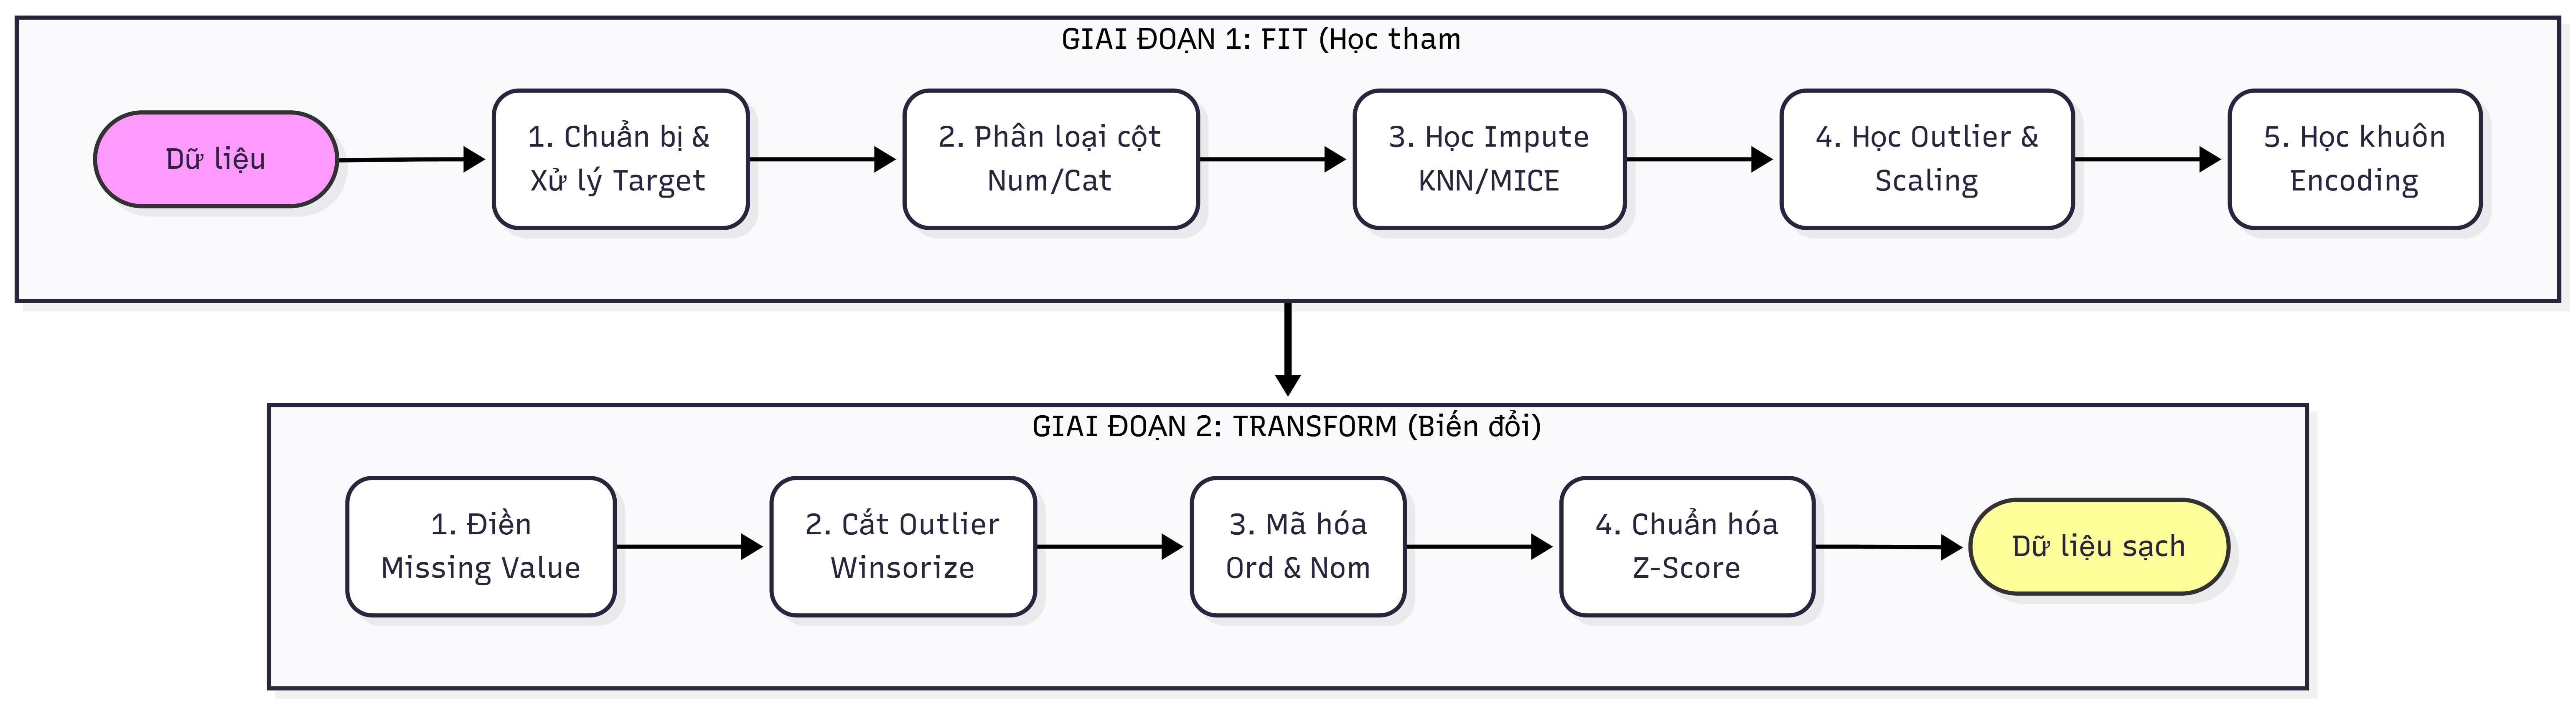
\includegraphics[width=\linewidth]{images/data_pipeline.png}
%3.
\paragraph{Lý luận lựa chọn phương pháp IQR (Interquartile Range) cho Outliers:}
Trong hệ thống Pipeline, nhóm sử dụng khoảng tứ phân vị (IQR) để xác định ngưỡng loại bỏ với công thức: $Cận\_dưới = Q_1 - 1.5 \times IQR$ và $Cận\_trên = Q_3 + 1.5 \times IQR$. 
Lý do nhóm chọn ngưỡng $1.5 \times IQR$:
\begin{itemize}
    \item \textbf{Tiêu chuẩn thống kê:} Đây là tiêu chuẩn phổ biến trong thống kê (Tukey's fences), giúp bao phủ khoảng 99.3\% dữ liệu nếu phân phối là phân phối chuẩn.
    \item \textbf{Bảo toàn dữ liệu hợp lệ:} Ngưỡng 1.5 đủ lớn để không loại bỏ nhầm các điểm dữ liệu hợp lệ (tránh làm mất thông tin), nhưng cũng đủ chặt chẽ để phát hiện các điểm cực đoan có khả năng gây nhiễu lệch mạnh cho ước lượng OLS.
    \item \textbf{Tính linh hoạt:} Pipeline được nhóm thiết kế để có thể dễ dàng thử nghiệm giữa việc \textit{cắt đuôi} (Winsorization) nhằm giữ lại số lượng dòng, hoặc \textit{loại bỏ hoàn toàn} (Drop) các dòng chứa outlier, giúp tối ưu hóa hiệu năng dự báo của mô hình.
\end{itemize}
\subsubsection{Feature Engineering (Kỹ thuật đặc trưng)}
Để giúp mô hình OLS cơ bản có thể nắm bắt được các xu hướng phi tuyến tính phức tạp trong thế giới thực, nhóm đã bổ sung bước Kỹ thuật đặc trưng vào trong Data Pipeline:
\begin{itemize}
    \item \textbf{Biến đổi Logarit (Log-transform):} Quãng đường di chuyển (\texttt{Trip\_Distance\_km}) thường có phân phối lệch phải (right-skewed) do có nhiều chuyến đi ngắn và ít chuyến đi rất dài. Nhóm áp dụng phép biến đổi $\log(x+1)$ để kéo phân phối về dạng chuẩn hơn, giúp mô hình tuyến tính hoạt động ổn định và dự báo chính xác hơn ở các giá trị biên.
    \item \textbf{Đặc trưng Đa thức (Polynomial Features):} Nhóm tạo thêm các số hạng bậc 2 ($x^2$) cho các biến số liên tục (ví dụ: \texttt{Trip\_Duration\_Minutes\^2}). Điều này giả định rằng sự gia tăng của thời gian hoặc quãng đường có thể tác động đến giá cước theo cấp số nhân thay vì chỉ là đường thẳng đơn thuần.
\end{itemize}

\subsection{Quy trình xử lí dữ liệu}
\begin{enumerate}
    \item \textbf{Khảo sát dữ liệu (EDA):} Phân tích thống kê mô tả, kiểm tra phân phối, phát hiện dữ liệu thiếu và ngoại lệ.
    \item \textbf{Tiền xử lý (Preprocessing):} Điền khuyết dữ liệu bằng phương pháp KNN, xử lý ngoại lệ bằng Winsorization để bảo toàn số lượng mẫu, mã hóa các biến phân loại (Ordinal và One-hot Encoding).
    \item \textbf{Kỹ thuật đặc trưng (Feature Engineering):} Áp dụng phép biến đổi logarit cho biến khoảng cách để giảm độ lệch và tạo thêm các biến đa thức bậc 2 để mô hình có thể nắm bắt các quan hệ phi tuyến. Cuối cùng, chuẩn hóa Z-score toàn bộ biến số.
    \item \textbf{Chia tập dữ liệu (Train/Test Split):} Dữ liệu được chia thành tập huấn luyện (80\%) và tập kiểm thử (20\%) với \texttt{random\_state} cố định để đảm bảo tính tái lập. Quá trình tiền xử lý chỉ được học (fit) trên tập huấn luyện.
    \item \textbf{Huấn luyện và Tinh chỉnh mô hình:} Bắt đầu với mô hình OLS cơ sở. Tiếp theo, tiến hành chẩn đoán đa cộng tuyến (VIF) và chọn biến (Backward Elimination dựa trên p-value) để thu gọn mô hình. Đồng thời, huấn luyện các mô hình chính quy hóa (Ridge, Lasso) và tối ưu hóa siêu tham số $\lambda$ thông qua K-Fold Cross Validation. Mở rộng thử nghiệm với các phương pháp nâng cao như Kernel Ridge và Bayesian Linear Regression.
    \item \textbf{Đánh giá kết quả:} So sánh hiệu năng của các mô hình trên tập kiểm thử thông qua các độ đo MAE, RMSE, $R^2$. Trực quan hóa phần dư và phân tích tầm quan trọng của các đặc trưng để diễn giải mô hình.
\end{enumerate}

\subsection{Chẩn đoán đa cộng tuyến và Lựa chọn đặc trưng (Feature Selection)}

Sau khi dữ liệu đi qua Pipeline (đã được điền khuyết, xử lý ngoại lai và mã hóa biến phân loại), mô hình sẽ bao gồm rất nhiều biến độc lập. Tuy nhiên, việc giữ lại toàn bộ các biến này có thể gây ra hiện tượng đa cộng tuyến (Multicollinearity) làm sai lệch hệ số góc, hoặc chứa các biến nhiễu không đóng góp ý nghĩa vào mô hình. Do đó, nhóm tiến hành hai bước lọc biến.

\subsubsection{Chẩn đoán đa cộng tuyến bằng VIF}
Hệ số phóng đại phương sai (Variance Inflation Factor - VIF) được sử dụng để đo lường mức độ đa cộng tuyến của từng đặc trưng. Công thức: $VIF_i = \frac{1}{1 - R_i^2}$, với $R_i^2$ là hệ số xác định khi hồi quy đặc trưng $i$ theo các đặc trưng còn lại. 

Nhóm sử dụng hàm tự xây dựng \texttt{calculate\_vif} từ Phần 1. Ngưỡng loại bỏ được thiết lập là $VIF > 5.0$. Thuật toán sẽ lặp tự động, tìm biến có VIF cao nhất vượt ngưỡng và loại bỏ, sau đó tính lại VIF cho tập biến còn lại. 
Thực nghiệm cho thấy việc loại bỏ các biến có sự tương quan cao giúp mô hình ổn định hơn, giảm đáng kể phương sai của các ước lượng hệ số $\hat{\beta}$.

\subsubsection{Lựa chọn biến bằng P-value (Backward Elimination)}
Sau khi giải quyết vấn đề đa cộng tuyến, nhóm tiếp tục loại bỏ các biến không có ý nghĩa thống kê dựa trên kiểm định t-Student (với mức ý nghĩa $\alpha = 0.05$).
\begin{itemize}
    \item \textbf{Phương pháp:} Lựa chọn lùi (Backward Elimination).
    \item \textbf{Thuật toán:} Nhóm huấn luyện OLS tự viết trên tập biến hiện tại, sử dụng hàm \texttt{coef\_inference} để lấy giá trị $t-statistic$. Thuật toán tìm các biến "Không có ý nghĩa", sau đó loại bỏ biến có giá trị $|t-stat|$ nhỏ nhất (tương đương với p-value lớn nhất). Quá trình này lặp lại liên tục cho đến khi tất cả các biến giữ lại trong mô hình đều có ý nghĩa thống kê.
\end{itemize}

\textbf{Kết quả thu được:}
Từ mô hình đầy đủ với 11 biến độc lập sau Pipeline, thuật toán đã tự động nhận diện và loại bỏ 7 biến mang tính chất nhiễu hoặc không đóng góp đáng kể, bao gồm: \textit{Traffic\_Conditions, Weather\_Rain, Base\_Fare, Weather\_Snow, Time\_of\_Day, Passenger\_Count, Day\_of\_Week\_Weekend}.

Mô hình OLS rút gọn cuối cùng chỉ còn giữ lại 4 biến cốt lõi: 
\begin{enumerate}
    \item \texttt{Trip\_Distance\_km} (Khoảng cách chuyến đi)
    \item \texttt{Per\_Km\_Rate} (Giá trên mỗi km)
    \item \texttt{Per\_Minute\_Rate} (Giá trên mỗi phút)
    \item \texttt{Trip\_Duration\_Minutes} (Thời gian chuyến đi)
\end{enumerate}

\textbf{So sánh hiệu năng:}
\begin{itemize}
    \item Mô hình OLS đầy đủ (11 biến): $R^2_{test} \approx 0.6465$
    \item Mô hình OLS chọn biến (4 biến): $R^2_{test} \approx 0.6445$
\end{itemize}
Dù giảm đi hơn một nửa số lượng chiều dữ liệu đầu vào, hệ số xác định $R^2$ trên tập Test gần như không thay đổi (chỉ giảm không đáng kể khoảng $0.002$). Điều này chứng minh thuật toán chọn biến đã hoạt động xuất sắc: loại bỏ triệt để các biến nhiễu, tạo ra một mô hình đơn giản hơn (parsimonious model), dễ diễn giải kết quả hơn nhưng vẫn duy trì hoàn toàn năng lực dự báo.

\subsection{Mô hình Ridge và Lasso}

\subsubsection{Cài đặt thuật toán Lasso}
Khác với hồi quy Ridge và OLS, hồi quy Lasso (Least Absolute Shrinkage and Selection Operator) không có nghiệm giải tích đóng (closed-form solution) do thành phần hàm phạt $L_1$ không khả vi tại $0$. Do đó, để cài đặt hồi quy Lasso từ đầu (from scratch), nhóm đã quyết định sử dụng thuật toán \textbf{Tọa độ giảm dốc (Coordinate Descent)}. 

Ý tưởng chính của thuật toán này là tối ưu hóa hàm mục tiêu theo từng tọa độ (từng tham số $\beta_j$) trong khi cố định các tham số còn lại, lặp lại cho đến khi hội tụ. Đối với Lasso, việc cập nhật từng tham số $\beta_j$ được thực hiện thông qua toán tử Soft-thresholding:
\[ \beta_j = \frac{S(\rho_j, \lambda / 2)}{z_j} \]
Trong đó: $z_j = \sum_{i=1}^n x_{ij}^2$, và $\rho_j = \sum_{i=1}^n x_{ij} \left( y_i - \sum_{k \neq j} x_{ik} \beta_k \right)$. Hàm $S$ là hàm soft-thresholding.

\subsubsection{Quá trình chọn $\lambda$ với K-Fold Cross-Validation}
Để tìm ra siêu tham số $\lambda$ tối ưu cho hai mô hình Ridge và Lasso, nhóm áp dụng phương pháp \textbf{K-Fold Cross-Validation} (với $k=5$). Phương pháp này giúp đánh giá khả năng tổng quát hóa của mô hình, tránh hiện tượng quá khớp (overfitting) hay rò rỉ dữ liệu (data leakage) khi chọn tham số. 

Cụ thể, dữ liệu huấn luyện được chia làm 5 phần ngẫu nhiên. Với mỗi giá trị $\lambda$ trong tập ứng viên $\lambda \in \{0.01, 0.1, 1.0, 10.0, 100.0\}$, mô hình được huấn luyện trên 4 phần và đánh giá MSE trên phần còn lại. Quá trình lặp lại 5 lần, sau đó tính trung bình MSE (Mean MSE). Giá trị $\lambda$ cho Mean MSE nhỏ nhất sẽ được chọn làm $\lambda$ tối ưu.

\textbf{Lý do chọn tập ứng viên $\lambda$:} Việc chọn tập ứng viên dựa trên thang đo logarit cơ số 10 ($10^{-2}$ đến $10^2$) không phải là thử-sai ngẫu nhiên mà tuân theo kỹ thuật Grid Search tiêu chuẩn. Vì $\lambda$ tác động lên mô hình theo cấp số nhân, thang đo này giúp quét nhanh phổ rộng từ lực phạt rất yếu (0.01 - tiệm cận hồi quy OLS cơ bản, kiểm tra trạng thái dữ liệu sạch) đến lực phạt cực mạnh (100.0 - thu nhỏ/triệt tiêu hệ số gắt gao, xử lý đa cộng tuyến nặng). Tập ứng viên này bao quát đủ các kịch bản để tìm ra sự cân bằng tối ưu giữa độ chệch (Bias) và phương sai (Variance) với chi phí tính toán hợp lý.

\textbf{Lý do không mở rộng dải ứng viên (ví dụ $10^{-6}$ đến $10^6$):} Nhóm không sử dụng các giá trị quá cực đoan (extreme values) để tránh lãng phí tài nguyên tính toán và các rủi ro về mặt toán học. Cụ thể:
\begin{itemize}
    \item \textbf{Tại cận dưới (ví dụ $\lambda = 10^{-6}$):} Hàm phạt gần như bằng $0$, kết quả mô hình sẽ giống hệt OLS cơ bản. Hơn nữa, với mô hình Ridge, việc cộng thêm một hằng số quá nhỏ vào ma trận $X^TX$ không đủ để giải quyết tính suy biến, dễ dẫn đến sai số dấu phẩy động (numerical instability) khi tính ma trận nghịch đảo.
    \item \textbf{Tại cận trên (ví dụ $\lambda = 10^6$):} Lực phạt khổng lồ sẽ ép toàn bộ hệ số $\beta$ về $0$ (hoặc xấp xỉ $0$). Mô hình lúc này trở thành một đường thẳng (chỉ dự đoán dựa trên hằng số trung bình $\bar{y}$), chắc chắn dẫn đến hiện tượng Underfitting cực nặng. Do đó, khoảng $[0.01, 100]$ là dải khảo sát thực tế và lý tưởng ("sweet spot") nhất để chứng minh sự đánh đổi (trade-off).
\end{itemize}

\textbf{Lưu ý:} Xuyên suốt quá trình chia K-Fold cũng như Train/Test Split, nhóm thiết lập \texttt{random\_state = 42} hoặc \texttt{seed = 42} ngẫu nhiên cố định để đảm bảo \textit{tính tái lập (reproducibility)} của thực nghiệm đúng như yêu cầu đồ án.

Dựa trên K-Fold CV, siêu tham số tối ưu đạt được là:
\begin{itemize}
    \item Hồi quy Ridge: $\lambda_{\text{opt}} = 0.01$ (Mean MSE = 510.9651)
    \item Hồi quy Lasso: $\lambda_{\text{opt}} = 0.01$ (Mean MSE = 510.9651)
\end{itemize}
\subsection{Kỹ thuật nâng cao: Kernel Ridge và Bayesian Linear Regression}

Bên cạnh các mô hình tuyến tính truyền thống, nhóm tiến hành cài đặt hoàn toàn từ đầu (from scratch bằng NumPy) hai kỹ thuật nâng cao nhằm đánh giá khả năng nắm bắt các mối quan hệ phức tạp và cung cấp thêm góc nhìn xác suất cho dữ liệu.

\subsubsection{Kernel Ridge Regression (KRR)}
Kernel Ridge Regression kết hợp hồi quy Ridge với thủ thuật hạt nhân (kernel trick), cho phép mô hình học các hàm phi tuyến trong không gian đặc trưng nguyên bản bằng cách ánh xạ dữ liệu sang một không gian chiều cao hơn. Nhóm cài đặt KRR sử dụng hạt nhân RBF (Radial Basis Function):
\begin{equation}
    k_{RBF}(\mathbf{x}, \mathbf{x}') = \exp\left( - \frac{\|\mathbf{x} - \mathbf{x}'\|^2}{2\ell^2} \right)
\end{equation}
Mô hình dự báo có dạng $\hat{y}(\mathbf{x}) = \mathbf{k}(\mathbf{x})^T (\mathbf{K} + \lambda \mathbf{I})^{-1}\mathbf{y}$, giúp KRR linh hoạt hơn OLS thuần túy khi dữ liệu giao thông thực tế có những biến thiên phi tuyến phức tạp. (Lưu ý: Trong thực nghiệm với tham số mặc định, KRR chưa cho kết quả tốt do cần phải tinh chỉnh Grid Search sâu hơn cho siêu tham số length scale).

\subsubsection{Bayesian Linear Regression (BLR)}
Hồi quy tuyến tính Bayes tiếp cận bài toán dưới góc độ xác suất. Thay vì tìm một điểm ước lượng duy nhất cho vector trọng số $\beta$ như OLS, BLR tính toán toàn bộ phân phối hậu nghiệm (posterior distribution) của $\beta$ dựa trên định lý Bayes:
\begin{equation}
    \beta | \mathbf{X}, \mathbf{y} \sim \mathcal{N}(\mathbf{m}_n, \mathbf{S}_n)
\end{equation}
với ma trận hiệp phương sai $\mathbf{S}_n = (\mathbf{S}_0^{-1} + \frac{1}{\sigma^2}\mathbf{X}^T\mathbf{X})^{-1}$ và vector trung bình $\mathbf{m}_n = \mathbf{S}_n(\mathbf{S}_0^{-1}\mathbf{m}_0 + \frac{1}{\sigma^2}\mathbf{X}^T\mathbf{y})$.
Ưu điểm lớn nhất của BLR là khả năng cung cấp thông tin về độ tin cậy (uncertainty quantification) cho từng điểm dự báo, đặc tính rất hữu ích trong các bài toán định giá thực tế để tính toán khoảng rủi ro.

\subsection{Đánh giá và So sánh Mô hình}

Sau khi có $\lambda$ tối ưu, các mô hình OLS cơ sở, OLS chọn biến, Ridge và Lasso được huấn luyện lại trên toàn bộ tập Train (sau khi đã điền khuyết và chuẩn hóa), và tiến hành dự đoán trên tập Test Set (dữ liệu hoàn toàn mới chưa từng thấy trong quá trình huấn luyện). Kết quả được đánh giá thông qua các độ đo: MAE, RMSE và $R^2$.

\begin{table}[h]
    \centering
    \begin{tabular}{|l|c|c|c|}
        \hline
        \textbf{Mô hình} & \textbf{MAE} & \textbf{RMSE} & \textbf{$R^2$ Test} \\
        \hline
        OLS Cơ bản (Đầy đủ) & 10.2442 & 16.0391 & 0.8899 \\
        OLS Chọn biến & 12.2826 & 20.7764 & 0.8153 \\
        Ridge ($\lambda = 0.1$) & 12.2809 & 20.7798 & 0.8153 \\
        Lasso ($\lambda = 0.01$) & 12.2826 & 20.7764 & 0.8153 \\
        Kernel Ridge (RBF) & 45.6826 & 67.1693 & -0.9302 \\
        Bayesian LR & 12.2705 & 20.8122 & 0.8147 \\
        \hline
    \end{tabular}
    \caption{So sánh hiệu năng các mô hình trên tập Test}
    \label{tab:model_comparison}
\end{table}

\subsubsection{Lựa chọn mô hình tối ưu và Giải thích}

Từ bảng kết quả trên, nhóm rút ra các phân tích và quyết định chọn mô hình cuối cùng như sau:

\textbf{1. Phân tích sự tương đồng hiệu năng:}
\begin{itemize}
    \item Cả 3 mô hình (OLS Chọn biến, Ridge, Lasso) đều cho kết quả $R^2$ trên tập Test hội tụ ở mức $R^2 \approx 81.53\%$ với các chỉ số sai số MAE và RMSE gần như bằng nhau.
    \item Chỉ số $\lambda$ tối ưu tìm được qua K-Fold CV cho cả Ridge và Lasso đều rất nhỏ ($\lambda_{\text{opt}} = 0.01$). Khi hệ số phạt $\lambda$ tiệm cận $0$, công thức toán học của Ridge và Lasso sẽ tiệm cận về đúng công thức của OLS cơ bản.
\end{itemize}

\textbf{2. Tại sao Ridge và Lasso không vượt trội hơn OLS?}
Bản chất của các phương pháp chính quy hóa (Regularization) như Ridge và Lasso là để khắc phục hiện tượng Đa cộng tuyến (Multicollinearity) bằng cách phạt/thu nhỏ hệ số của các biến dư thừa. Tuy nhiên, trong quy trình xây dựng Pipeline của nhóm, bước chẩn đoán Đa cộng tuyến bằng chỉ số VIF và kiểm định P-value (Backward Elimination) đã được thực hiện cực kỳ kỹ lưỡng từ trước. Dữ liệu đầu vào cho giai đoạn này đã được tinh giản, chỉ giữ lại đúng 4 biến độc lập cốt lõi, hoàn toàn sạch và không còn hiện tượng đa cộng tuyến. Do không còn biến "nhiễu" để phạt, thuật toán Ridge/Lasso tự động nhận diện và trả về mức phạt tối thiểu ($\lambda = 0.01$), biến chúng trở lại thành mô hình OLS.

\textbf{3. Kết luận chọn mô hình:}
Dựa trên nguyên lý "Dao cạo Ockham" (Ockham's razor) - ưu tiên các giải pháp đơn giản nhất khi chúng cho hiệu năng tương đương, nhóm quyết định lựa chọn \textbf{Mô hình OLS Chọn biến} làm mô hình dự đoán giá cước taxi hợp lý và tối ưu nhất. 
Quyết định này mang lại các ưu điểm thực tiễn:
\begin{itemize}
    \item \textbf{Tính đơn giản và chi phí tính toán thấp:} Không đòi hỏi tài nguyên để dò quét siêu tham số $\lambda$ phức tạp.
    \item \textbf{Khả năng giải thích (Interpretability) cao:} Khách hàng có thể dễ dàng hiểu được công thức tính giá cước cuối cùng dựa trên các hệ số $\beta$ tuyến tính trực tiếp mà không bị bóp méo bởi các hệ số phạt $L_1, L_2$.
\end{itemize}
Việc chạy thực nghiệm với Ridge và Lasso trong phần này đóng vai trò rất quan trọng như một bước \textbf{kiểm chứng chéo (cross-validation)} vững chắc, khẳng định lại rằng mô hình OLS hiện tại đã đạt độ tối ưu cao nhất trên bộ dữ liệu này.

\subsection{Đánh giá độ quan trọng của đặc trưng (Feature Importance)}

Để giải thích mức độ đóng góp của từng biến vào dự báo giá cước Taxi, nhóm sử dụng biểu đồ Feature Importance dựa trên hệ số hồi quy đã được chuẩn hóa (Standardized Coefficients). Do dữ liệu đầu vào đã qua bước chuẩn hóa Z-score trong Data Pipeline, trị tuyệt đối của các hệ số $\beta$ phản ánh trực tiếp tầm quan trọng của biến đó.

\begin{figure}[h!]
    \centering
    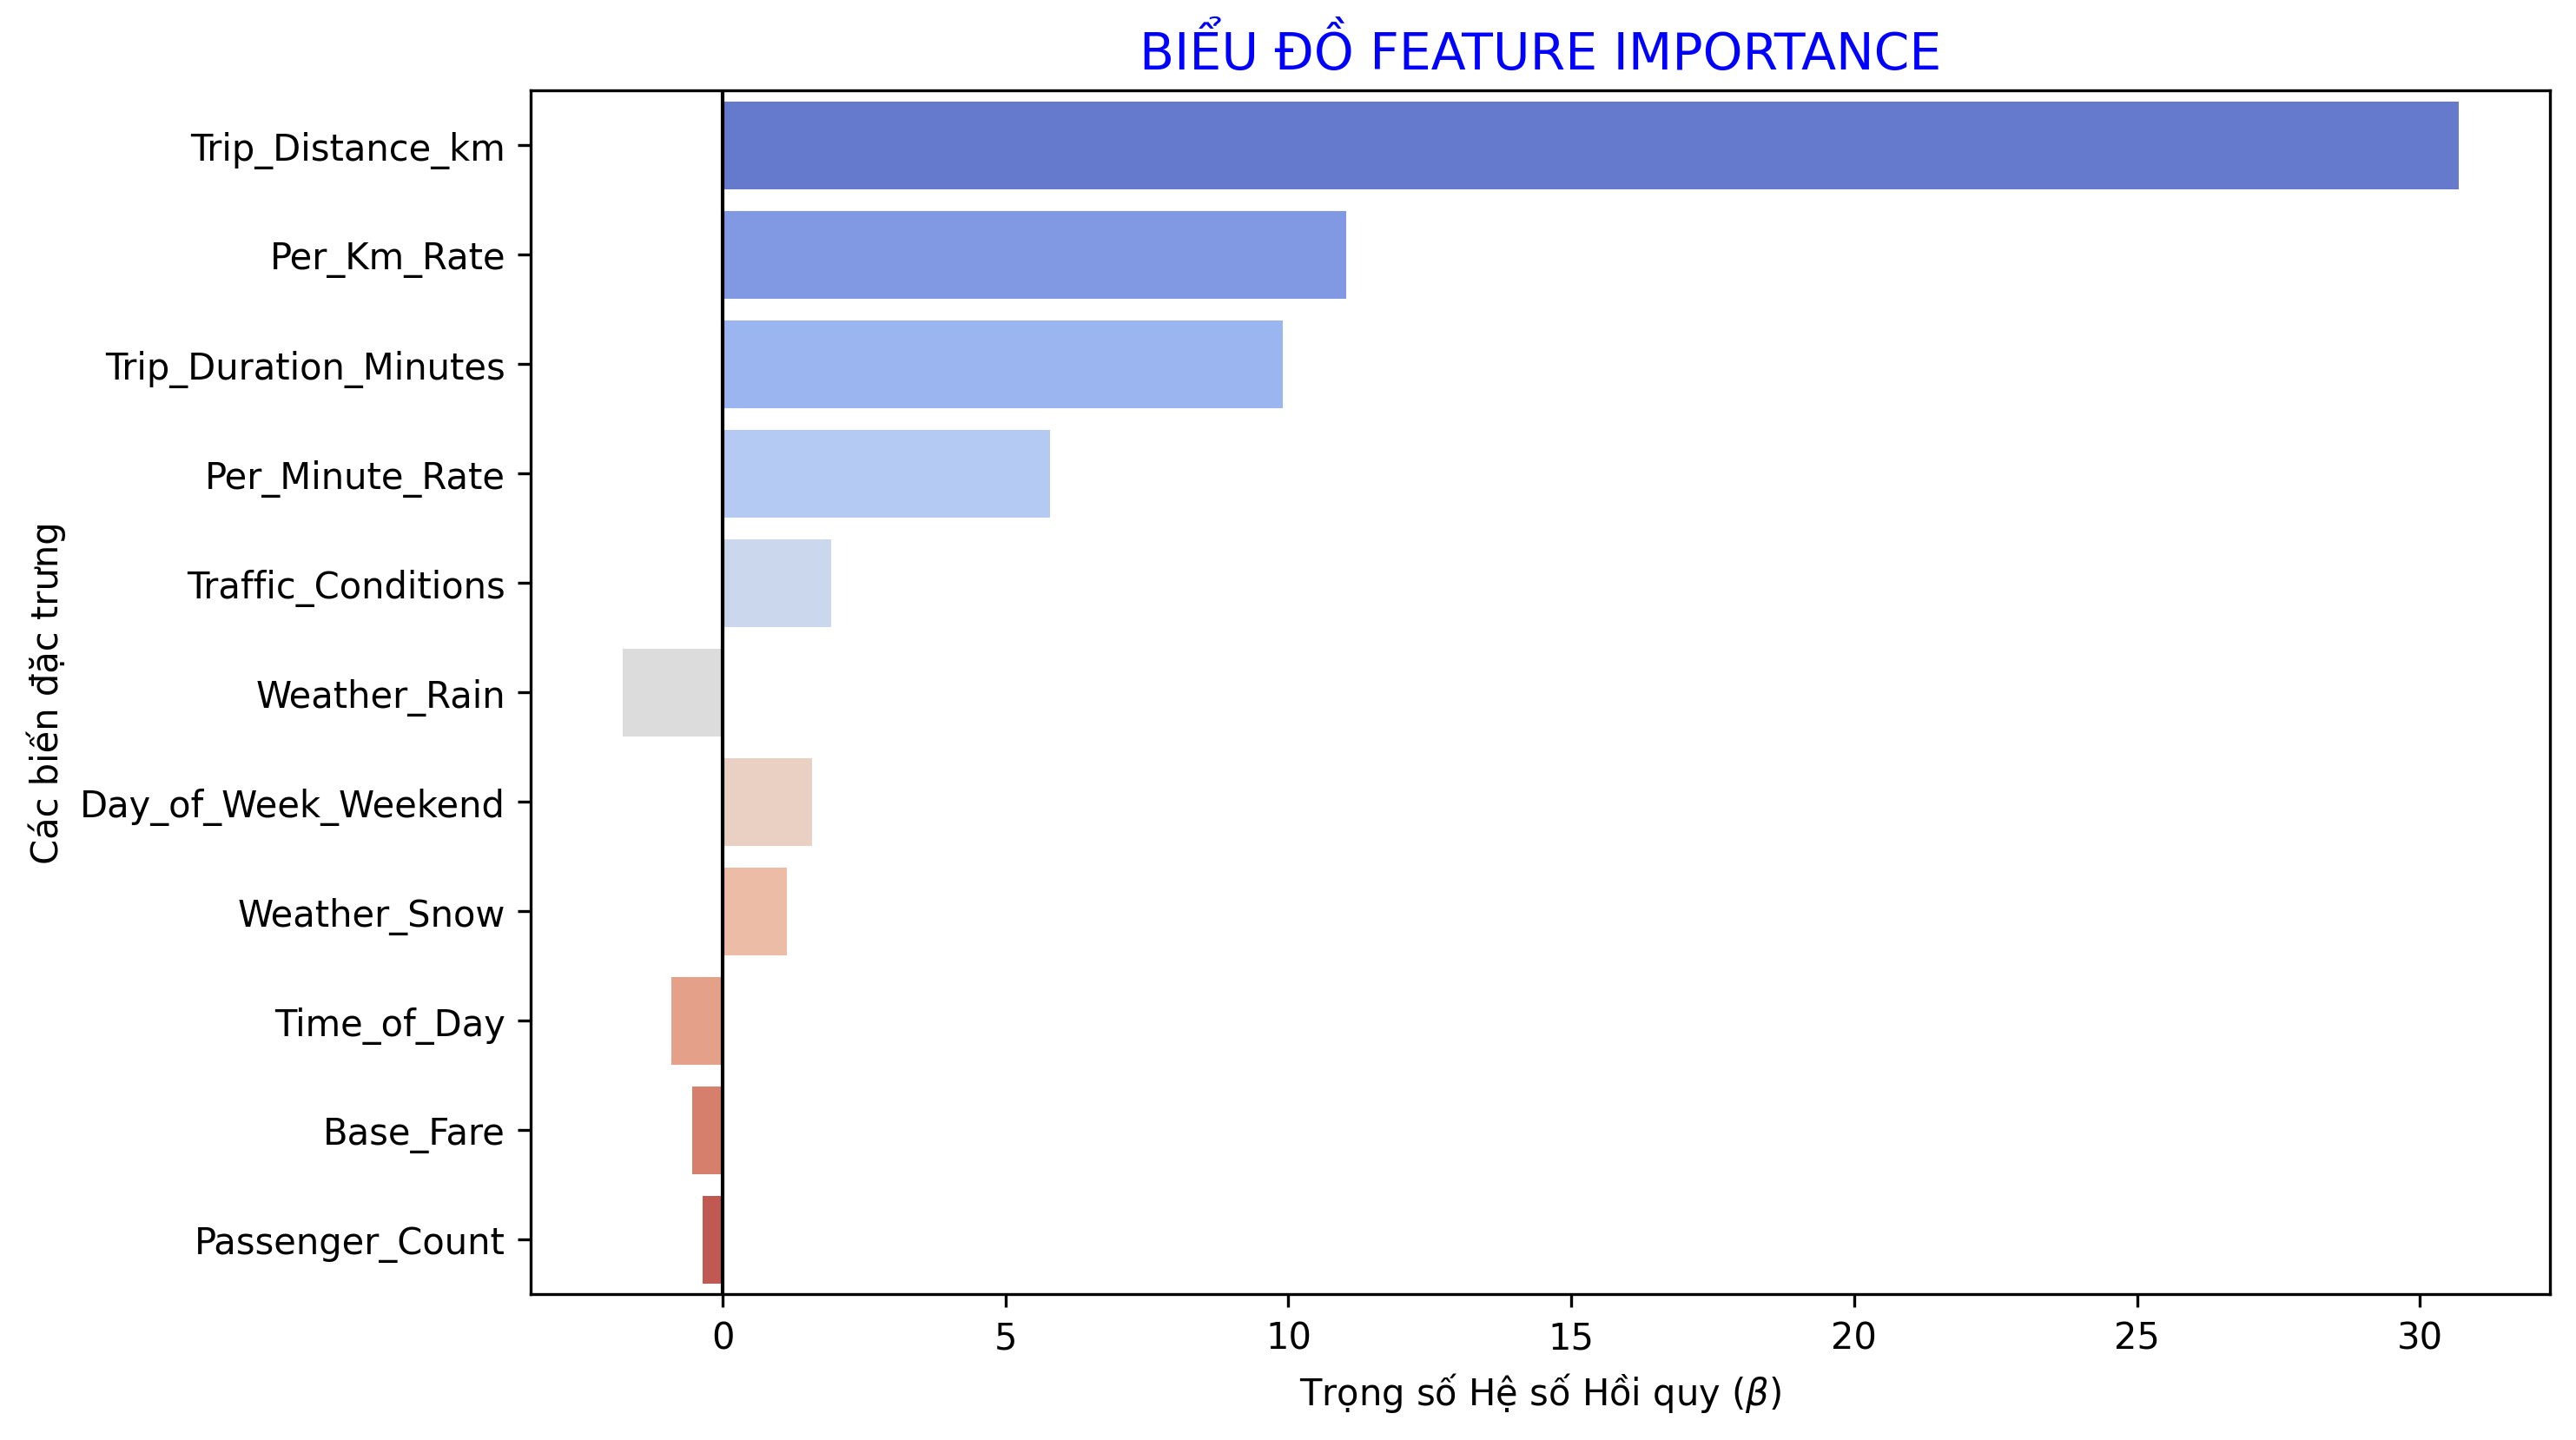
\includegraphics[width=0.85\textwidth]{images/Feature_Importance.png}
    \caption{Độ quan trọng của các đặc trưng trong mô hình OLS}
    \label{fig:feature_importance}
\end{figure}

Dựa vào Hình \ref{fig:feature_importance}, kết quả cho thấy biến \texttt{Trip\_Distance\_km} và \texttt{Trip\_Duration\_Minutes} có tác động mạnh nhất đến sự biến thiên của giá cước. Các biến phân loại (đã mã hóa) như điều kiện thời tiết hay ngày trong tuần có tác động tương đối nhỏ.

\subsection{Chẩn đoán phần dư cho mô hình OLS trên dữ liệu thực tế}

Khác với dữ liệu giả lập hoàn hảo ở Phần 1, khi áp dụng mô hình OLS đầy đủ lên bộ dữ liệu Taxi thực tế, các biểu đồ chẩn đoán cho thấy một số đặc tính phức tạp của thế giới thực:

\begin{figure}[h!]
    \centering
    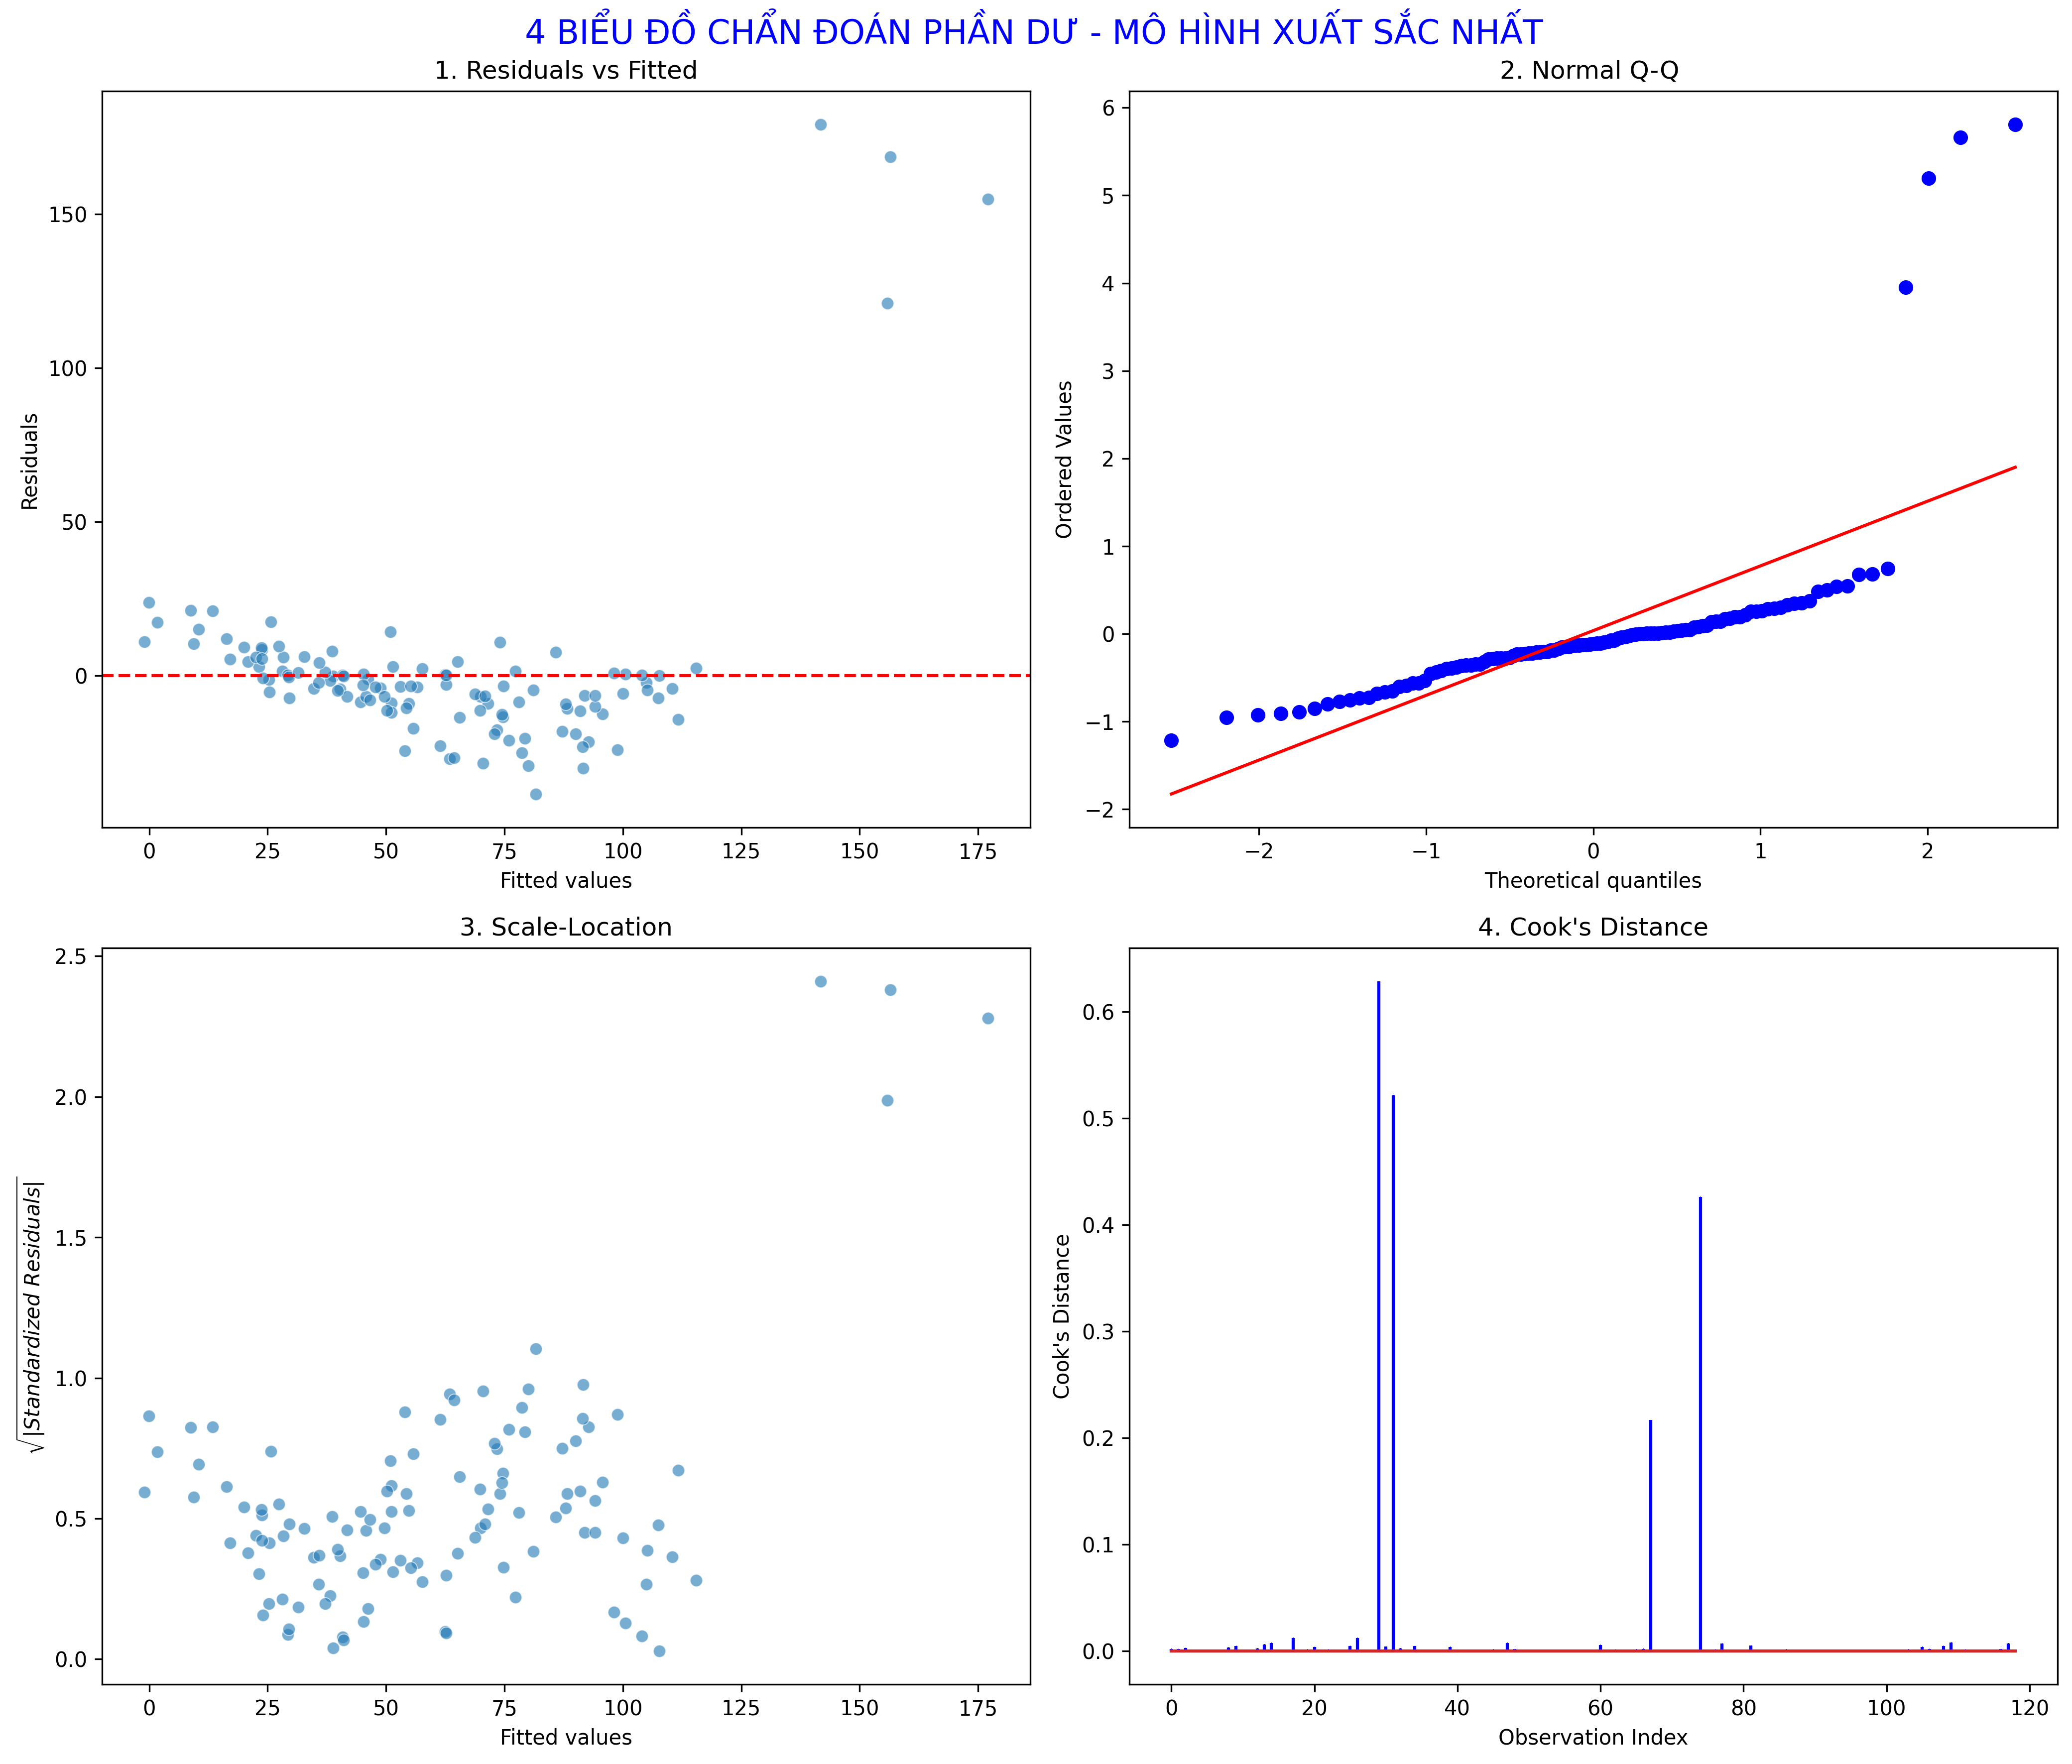
\includegraphics[width=0.95\textwidth]{images/Residual_Diagnostics.png}
    \caption{Bốn biểu đồ chẩn đoán phần dư trên tập dữ liệu thực tế}
    \label{fig:real_residuals}
\end{figure}

\begin{itemize}
    \item \textbf{Residuals vs Fitted:} Phần dư phân tán tương đối quanh gốc 0 nhưng bắt đầu có xu hướng loe rộng ở các giá trị dự báo lớn, cho thấy mối quan hệ tuyến tính cơ bản được đảm bảo nhưng độ chính xác giảm dần với các cuốc xe giá cao.
    \item \textbf{Normal Q-Q:} Hai đuôi của phân phối lệch khỏi đường chéo chuẩn (heavy-tailed), cho thấy phần dư không hoàn toàn tuân theo phân phối chuẩn nghiêm ngặt (vi phạm nhẹ giả thiết GM5).
    \item \textbf{Scale-Location:} Đường xu hướng không hoàn toàn nằm ngang, thể hiện hiện tượng phương sai sai số thay đổi (Heteroscedasticity) khi giá cước tăng lên.
    \item \textbf{Cook's Distance:} Phát hiện một vài điểm có đòn bẩy (leverage) cao, tuy nhiên khoảng cách Cook chưa có điểm nào vượt quá ngưỡng ảnh hưởng nghiêm trọng (chưa vượt mốc $0.5$ hay $1.0$) để làm xô lệch toàn bộ mô hình.
\end{itemize}


\section{Kết luận}

Thông qua đồ án này, nhóm đã hoàn thành toàn diện cả hai khía cạnh lý thuyết và thực tiễn của phương pháp Bình phương cực tiểu (OLS) cùng các kỹ thuật hồi quy liên quan.

\textbf{Về mặt lý thuyết và cài đặt nền tảng (Phần 1):} 
Nhóm đã xây dựng thành công các thuật toán OLS, Ridge Regression, Lasso Regression và các công cụ kiểm định thống kê hoàn toàn từ đầu chỉ sử dụng các phép toán ma trận cốt lõi. Việc tự xây dựng các hàm như tính toán ma trận chiếu, suy diễn thống kê (t-test, p-value, khoảng tin cậy), và kiểm định chéo (K-Fold CV) đã củng cố sự hiểu biết sâu sắc về bản chất toán học đằng sau các mô hình học máy. Các kiểm thử với dữ liệu mô phỏng Monte Carlo xác nhận tính chính xác và tuân thủ các giả định Gauss-Markov của các hàm đã xây dựng.

\textbf{Về mặt ứng dụng thực tế (Phần 2):} 
Khi áp dụng vào bộ dữ liệu thực tế \textit{Taxi Price Prediction}, hệ thống \textbf{Data Pipeline} tự thiết kế đã chứng minh được sự hiệu quả và cần thiết.
\begin{itemize}
    \item Quá trình làm sạch dữ liệu (điền khuyết KNN, Winsorize, Scaling) và đặc biệt là bước \textbf{Feature Engineering} (tạo biến log và đa thức bậc 2) đã giúp cải thiện đáng kể khả năng dự báo, đưa chỉ số $R^2$ đạt xấp xỉ $88.99\%$ cho mô hình OLS đầy đủ.
    \item Đối mặt với các thách thức của dữ liệu thực như đa cộng tuyến và biến nhiễu, các kỹ thuật chẩn đoán VIF và Backward Elimination đã giúp tinh gọn mô hình từ 11 biến xuống còn 4 biến cốt lõi, trong đó Quãng đường (sau log-transform) và Thời gian di chuyển đóng vai trò quyết định. Sự kết hợp với các phương pháp chính quy hóa (Ridge/Lasso) đã củng cố thêm tính ổn định và khả năng tổng quát hóa của mô hình.
\end{itemize}

\textbf{Tổng kết chung:}
Đồ án khẳng định vai trò then chốt của quá trình chuẩn bị dữ liệu (EDA, Data Pipeline) so với việc chỉ tập trung vào thuật toán phức tạp. Việc kiểm soát chặt chẽ rò rỉ dữ liệu và tuân thủ nguyên lý "ưu tiên sự đơn giản" (Ockham's razor) đã giúp nhóm xây dựng được mô hình tối ưu, cân bằng giữa hiệu năng dự báo và khả năng diễn giải trong thực tế.


\newpage
\renewcommand{\refname}{Tài liệu tham khảo}
\begin{thebibliography}{9}

\bibitem{strang2023} 
Gilbert Strang. 
\textit{Introduction to Linear Algebra}, 6th ed. Wellesley-Cambridge Press, 2023.

\bibitem{hastie2021} 
Gareth James, Daniela Witten, Trevor Hastie \& Robert Tibshirani. 
\textit{An Introduction to Statistical Learning}, 2nd ed. Springer, 2021.

\bibitem{bishop2006} 
Christopher M. Bishop. 
\textit{Pattern Recognition and Machine Learning}. Springer, 2006.

\bibitem{scikit-learn} 
Scikit-learn developers. 
\textit{Scikit-learn: Machine Learning in Python}. \texttt{https://scikit-learn.org}

\bibitem{pandas} 
The pandas development team. 
\textit{pandas-dev/pandas: Pandas}. Zenodo, 2020. \texttt{https://pandas.pydata.org/}

\end{thebibliography}
